% modello documentale di nicola santi ego@nicolasanti.it



\documentclass[pdftex,a4paper,12pt,twoside,openright]{book}

\usepackage[italian]{babel}
\usepackage[T1]{fontenc}
\usepackage[utf8]{inputenc}
\usepackage{indentfirst}

% decora i titoli dei capitoli
\usepackage[Lenny]{fncychap}

% inserimento di immagini come effetto indesiderato
% produce solo pdf come output e non più dvi.
\usepackage[pdftex]{graphicx}
\DeclareGraphicsExtensions{.pdf,.png,.jpg}
\graphicspath{{./images/}}

\newcommand{\HRule}{\rule{\linewidth}{0.5mm}}

% floatings, caption laterali
\usepackage{sidecap}

% immagini avvolte all'interno del testo
\usepackage{wrapfig}

% citazioni in stile Hardvare
\usepackage{natbib}
\bibpunct{(}{)}{;}{a}{,}{,}

% forza LaTeX ad una spaziatura fra parole non inglese
\frenchspacing 

% per inserire del codice sorgente
\usepackage{listings}
\usepackage{color}
\definecolor{light-gray}{gray}{0.95}


\lstnewenvironment{java}[1][]
{\lstset{language=Java,numbers=left, numberstyle=\tiny, stepnumber=2, numbersep=5pt,backgroundcolor=\color{light-gray},breaklines=true,breakatwhitespace=true,breakindent=0pt,basicstyle=\scriptsize,#1}}
{}

\lstnewenvironment{bash}[1][]
{\lstset{language=Bash,numbers=left, numberstyle=\tiny, stepnumber=2, numbersep=5pt,backgroundcolor=\color{light-gray},breaklines=true,breakatwhitespace=true,breakindent=0pt,basicstyle=\scriptsize,#1}}
{}

\lstnewenvironment{xml}[1][]
{\lstset{language=Xml,numbers=left, numberstyle=\tiny, stepnumber=2, numbersep=5pt,backgroundcolor=\color{light-gray},breaklines=true,breakatwhitespace=true,breakindent=0pt,basicstyle=\scriptsize,#1}}
{}



% indentazione del primo paragrafo
\setlength{\parindent}{18pt}

% serve per gestire le tabelle
\usepackage{array}
\usepackage{multirow}
\usepackage{booktabs}

% per inserire l'euro
\usepackage[official]{eurosym}

% liste più compatte
\usepackage{mdwlist}

% liste inline
\usepackage{paralist}

% miglioare i riferimenti
\usepackage[italian]{varioref}
%\def\reftextfaraway#1{a pagina~\pageref{#1}}%
%\def\reftextpagerange#1#2{nelle pagine~\pageref{#1}--\pageref{#2}}%

% hyper link in LaTex
\usepackage{html}

% indici
\usepackage{makeidx}
\makeindex

% un simpatico box

\usepackage{dashbox}

\newenvironment{nota}
{\rule{1ex}{1ex}\hspace{\stretch{1}}}
{\hspace{\stretch{1}}\rule{1ex}{1ex}}



\begin{document} 

%-----------TOP MATTER

%\title{Pojo's in action} 

%\author{Nicola Santi\\
%  Università di Bologna\\
%  \texttt{ego@nicolasanti.it}}
%\date{\today}

%\maketitle 
\begin{titlepage}
 
\begin{center}
 
 
% Upper part of the page

\includegraphics[width=0.40\textwidth]{regola-kit}\\[1cm]
 
\textsc{\LARGE }\\[1.5cm]
 
\textsc{\Large java ed il web per gente pratica }\\[0.5cm]
 
 % Title
\HRule \\[0.4cm]
{ \huge \bfseries scrivere con Regola}\\[0.4cm]
 
\HRule \\[1.5cm]

 
% Author and supervisor
\begin{minipage}{0.4\textwidth}
\begin{flushleft} \large
\emph{Autori:}\\
Nicola \textsc{Santi}, Marco \textsc{Rosi}
\end{flushleft}
\end{minipage}
\begin{minipage}{0.4\textwidth}
\begin{flushright} \large
\emph{Supervisore:} \\
Lorenzo \textsc{Bragaglia}
\end{flushright} 
\end{minipage}
 
\vfill
 
% Bottom of the page
{\large \today}
 
\end{center}
 
\end{titlepage}

% -----------TOC
\tableofcontents
%\listoffigures
%\listoftables





\addcontentsline{toc}{subsection}{Prefazione}

\subsection*{Prefazione}

\begin{bash}
La societ aperta e aperta a piu valori, a piu visioni del mondo filosofiche e a piu fedi religiose, ad una molteplicita di proposte per la soluzione di problemi concreti e alla maggior quantita di critica. La societa aperta e aperta al maggior numero possibile di idee e ideali differenti, e magari contrastanti. Ma, pena la sua autodissoluzione, non di tutti: la societ aperta e chiusa solo agli intolleranti.
(Karl R. Popper, La societa aperta e i suoi nemici, Vol. I, Platone totalitario, dalla IV di copertina.)
\end{bash}

Non credo sia necessario abbracciare in toto la posizione filosofica nota come Relativismo per cogliere di quanto varino costumi e valori anche solo viaggiando nel spazio oggi: ogni società è unica, ogni costume trova giustificazione nel contesto in cui si è formato ed in questa diversità e di questa diversità  si alimenta e prolifera il sapere umano. Se poi si azzardassero dei viaggi non solo nello spazio ma nelle profondità del tempo il nostro stupore si amplierebbe risalendo controcorrente il fiume dei secoli secoli. Il sistema di valori che assegna un  giudizio positivo di un condottiero militare quale Alessandro Magno come avrebbe giudicato il Mahatma Gandhi? Quale sono le imprese per cui un padre (poté e possa) essere orgoglioso dei propri figli? Quale il modo  etico di legiferare ed il concetto stesso di qualità di una casa od una vita intera come si è modificato attraversando anni di evoluzioni? Quale risposte possiate proporre a queste domande tutte dovranno, se non spiegare, scendere a compromessi con la variazione, la moda, il prendere atto che è tradizione che le cose cambino: è il panta rei di Eraclito, il tema eterno del divenire che procede spesso gradualmente mentre a volte in modo netto, traumatico. Ed è proprio lungo questa linea evanescente e discontinua che separa il nuovo corso (ancora impreciso e difficile da definire) dalla vecchia maniera (ancora presente ma senza più i favori del Tempo)  destinata a scomparire;  lungo questa linea che si dispongono schieramenti di persone in antitesi, a volte in conflitto aperto, cercando di lottare per quello in cui credono. Le une, come le altre senza alcuna garanzia di avere ragione e senza sfere di cristallo che li rinsaldino nelle loro convinzioni: solo passione, l'illuminisme ed il sentimento. Poca cosa, si dirà però è quello che è dato al genere umano ed è quanto basta in mano ad uomini e donne di valore.
Un esempio di questo genere di confronto si è avuto nel XIV secolo all'interno del mondo letterario nella penisola italica tra lingua latina e lingua volgare. Un intellettuale fiorentino destinato ad una fama mondiale immensa chiamato Dante Alighieri partecipò allo scontro e scrisse un saggio a titolo de vulgari eloquentia. Il testo curiosamente è scritto in latino (perché destinato a dotti ed intellettuali dell'epoca) ma sostiene l'importanza e la dignità della lingua volgare proprio contro il latino (ed il greco). Ecco un passaggio tradotto in volgare del primo libro:

I-i-4 Di queste due lingue la più nobile è la volgare: intanto perché è stata adoperata per prima dal genere umano; poi perché il mondo intero ne fruisce, benché sia differenziata in vocaboli e pronunce diverse; infine per il fatto che ci è naturale, mentre l'altra è, piuttosto, artificiale. 

Una difesa delle lingue apprese in modo naturale, dalle nostre madri, quando ancora bambini muoviamo i primi passi nel mondo ed impariamo a chiamare le cose con il nome che gli uomini hanno attribuito loro. La lingua che utilizziamo tutti i giorni nelle miserie del quotidiano ma anche la lingua con cui ci dichiariamo ai nostri amati, con cui consoliamo i nostri figli e con cui cerchiamo di riempire il silenzio dell'infinito stellato. La lingua che l'Alighieri avrebbe usato poi per scrivere i suoi sonetti e la sua Commedia dimostrando così come il volgare non avesse nulla da invidiare all'accademico latino in quanto ad espressività, completezza: una lingua aulica, forgiata dal basso ed utilizzata da gente comune così come da poeti e letterati per il lavoro quotidiano e la più alta poesia.

Nello sviluppo in Java si è presentata una situazione per diversi tratti simile al panorama letterario italiano del XIV secolo. Fino al 1998 (ed oltre) si utilizzava Java seguendo l'imperante tradizione della progettazione ad oggetti; costrutti linguistici e tecniche come l'ereditarietà ed il polimorfismo venivano utilizzate per affrontare e risolvere in modo eleganti i problemi affrontati. Ogni intervento era realizzato nella cornice teorica di principi come l'Open/Closed, il principio di inversione delle dipendenze, il principio di sostituzione di Liskov ad altri ancora oggi del tutto validi ed accreditati. Con l'esplosione poi del movimento dei design pattern (come riferimento Gof del 1995) la scrittura raggiunse livelli di raffinatezza elevatissimi con architetture complesse ma intuitive e facili da mantenere ed espandere; inoltre la capacità di descrivere problemi e soluzioni in modo universalmente accettato ampliarono la banda di comunicazione tra i le persone coinvolte nello sviluppo in modo inaudito. Annotare una classe come implementazione, ad esempio, del pattern Facade consentiva a chiunque di comprendere il problema affrontato (dare una vista semplificata di un sottosistema complesso) e la soluzione messa in piedi (una classe ritagliata sulle esigenze dei client). Si andava diffondendo un modo di utilizzare Java come linguaggio di pattern e questo consentì di progettare soluzioni incredibili e di spostare il discorso dell'analisi fino ai confini stessi della progettazione ad oggetti, cogliendone i limiti e proponendo soluzioni complementari note poi come progettazione orientata agli aspetti.
Proprio in questo contesto di ricerca febbrile e risultati poderosi che nel 1998 calano dall'alto delle torri di Sun (l'azienda che Java aveva inventato pochi anni prima) delle specifiche contenenti  le applicazioni serie, quelle destinate alle aziende che si propongono sfide impegnative sia come scalabilità che come manutenzione. Queste specifiche presero il nome di J2EE (ora si chiamano JEE) ed arrivarono come le tavole di pietra della legge di Mosè: ovvero contenevano la verità ed il giusto modo. Tutto quello che si era fatto e si faceva doveva cessare, mutare, adattarsi perché J2EE era la sola via corretta per affrontare problemi complessi. A distanza di 1700 anni si ripresentava aulica ed imposto dall'autorità la scrittura latina: ancora una volta artificiale, ancora una volta appannaggio di pochi intellettuali, ancora una volta scelta imposta.
In verità, mentre nei corsi universitari fiorivano corsi dedicati a J2EE,  nella pratica quotidiana il numero di applicazioni che lo utilizzava rappresentava un minoranza quasi esoterica. Infatti in pochi erano disposti ad accettare (o permettersi finanziariamente) i limiti che questo stack tecnologico imponeva; ad esempio non è mai stato possibile trovare un buon motivo per rinunciare all'ereditarietà. Così come è sempre parso innaturale la segregazione del modello all'interno dei confini degli EJB server senza poterli passare ai livelli di presentazione se non sotto forma di anemici delegati a nome DTO. Inoltre mentre i tempi di sviluppo salivano a causa delle lunghe attese per i riavvii degli application server si constatava con amarezza come J2EE rendesse difficile se non impossibile una metodologia di sviluppo nota come Test Driven Developement che aveva dato invece buona prova di sé nella creazione di applicazioni robuste.
A causa di questi, ed altri motivi, apparve di nuovo la linea effimera di separazione tra fazioni apposte e lo schieramento della lingua volgare fece il suo ritorno. Anche questa volta si presentava come un linguaggio naturale, costruito dal basso per risolvere problemi concreti ma capace di accettare e vincere le sfide più complesse delle applicazioni aziendali. Anche questa volta intellettuali capaci si schierarono in difesa del volgare. Tra questi Rod Johson che fornì gli strumenti per affrontare in modo elegante, efficace, sistematico ed economicamente vantaggioso le sfide offerte dalle applicazioni aziendali progettando e rilasciando come open source il framework chiamato Spring. La scelta dell'open source è stata fondamentale per il successo di Spring in quanto ha consentito di integrare assieme tutte le soluzioni che la comunità aveva realizzato in quegli anni come risposta a J2EE tra cui ricordo solo Hibernate ed iBatis ma potrei parlare delle librerie commons, struts, tomcat e molti altri. In contrasto con J2EE Spring si fece chiamare contenitore leggero (o invertito) ed i mattoni di cui si componeva lo sviluppo classi Pojo, ovvero Plain Old Java Object per rimarcarne la semplicità e la tradizione legata alla progettazione ad oggetti.
Il successo di mercato di Spring fu velocissimo ed imponente: applicazioni finanziarie, aeroportuali, governative, mediche, bancarie furono realizzate in tutto il mondo dimostrando l'efficacia del modello proposto. Il riscontro fu tale che la Sun stessa decise (tardivamente e parzialmente) di riadattare J2EE sottoponendolo ad una clamorosa inversione di orientamento architetturale  per spingerlo ad abbracciare temi come Pojo Programming ed iniezione delle dipendenze. La portata del dietro front fu tale che anche il nome cambio in JEE e tutto lo stack tecnologico ufficiale iniziò il percorso che Spring aveva inaugurato molti anni prima e che forse un giorno poterà i due antagonisti a somigliarsi al punto dal diventare di fatto la stessa cosa. Ma questo solo quando JEE recupererà il tempo perso e solo se Spring dovesse arrestare la sua evoluzione.


% -----------CAPITOLI
\chapter{Getting Started}

Questo capitolo è una cura per gli impazienti; seguendo le istruzioni dei paragrafi seguenti sarete in grado di installare e predisporre una prima applicazioni web con Regola.

\section{Installare Regola kit}
\index{installazione} 
Le applicazioni realizzate con Regola kit utilizzano Maven 2 per tutta la gestione del ciclo di build (compilazione, esecuzione dei test, creazione dei file war, \ldots). Quindi come prima cosa bisogna installare Maven 2 
scaricandolo dal sito \htmladdnormallink{maven.apache.org} {http://maven.apache.org} e seguendo le istruzioni.

Finita l'installazione di Maven 2 verificate che tutto sia andato a buon fine aprendo una console di terminale e lanciando il seguente comando.

\begin{bash}
nicola@casper:~# mvn -version
Maven version: 2.0.8
Java version: 1.6.0_03
OS name: "linux" version: "2.6.22-14-generic" arch: "i386" Family: "unix"
\end{bash}

Se tutto è corretto Maven 2 risponde al comando restituendo la sua versione, quella di Java ed infine alcune informazioni circa il sistema operativo in uso.

Regola kit non richiede nessuna installazione particolare (anche se è possibile scaricare un pacchetto contente documentazione e comandi di utilità): quindi finita l'installazione di Maven 2 siete pronti già per utilizzare Regola kit.


%\setlength{\fboxrule}{0.1pt} 
%\framebox[\width]{
%\begin{minipage}{0.9\textwidth}
\begin{nota}
Per maggiori informazioni su come installare Regola kit sulle vostre macchine di sviluppo si rimanda al capitolo  \vref{chap:installazione}.
\end{nota}
%\end{minipage}
%}


\section{Predisporre il database}
Per questo tutorial ipotizziamo di avere a disposizione un database di tipo MySql già installato sulla macchina dove intendiamo creare il progetto. Assicuratevi che il database stia funzionando e digitate il comando seguente:

\begin{bash}
nicola@casper:~# mysql -u root -p
\end{bash}

Vi troverete dentro la shell di amministrazione di MySql. Approfittatene per creare un nuovo database che sarà utilizzato dall'applicazione digitando il comando.

\begin{bash}
mysql> create database clienti;
\end{bash}

(Attenzione al punto e virgola in fondo al comando).
A questo punto non ci resta che creare anche l'utente utilizzato dalla nostra applicazione per accedere al database (nell'esempio porta il mio nome \emph{nicola}).

\begin{bash}
mysql> grant all on clienti.* to 'nicola'@'localhost';
\end{bash}

Bene, con il database abbiamo finito. Digitate questo ultimo comando per uscire dalla shell di amministrazione di MySql e passare al paragrafo seguente.

\begin{bash}
mysql> exit
\end{bash}

\begin{nota}
Regola kit è in grado di utilizzare diversi DBMS (ad esempio Oracle, Microsoft Sql, PostgreSQL, Hypersonic, \ldots). Per sapere come configurare la vostra applicazione per utilizzare DBMS diversi da MySql si rimanda al capitolo \vref{chap:persistenza}.
\end{nota}



\section{Creare un progetto con Regola kit}

Posizionatevi nella cartella dove volete creare il vostro nuovo progetto e digitate un comando simile al seguente con l'accortezza però di modificare il parametro gruopId (nell'esempio \emph{com.acme}) con il nome del vostro package di default ed il parametro  artifactId (nell'esempio  \emph{clienti}) con il nome del nuovo progetto.

\begin{bash}
nicola@casper:~# mvn archetype:create -DarchetypeGroupId=org.regola  \ 
-DarchetypeArtifactId=regola-jsf-archetype \
-DarchetypeVersion=1.1-SNAPSHOT -DgroupId=com.acme \
-DartifactId=clienti
\end{bash}

\emph{Attenzione: il comando qui sopra è riparito su diverse righe per chiarezza tipografica, deve invece essere digitato su una sola riga.}

La prima volta che lanciate questo comando Maven 2 scarica tutte le librerie necessarie (la cosa potrebbe prendere un po' di tempo) e crea una sotto cartella col nome del progetto (nell'esempio la cartella clienti). Il progetto è questo punto è già stato creato, posizioniatevi all'interno della cartella  \emph{clienti} col comando:

\begin{bash}
nicola@casper:~# cd clienti
\end{bash}


\section{Collegarsi al database}\label{sec:db-link}

Prima di lanciare la nostra nuova applicazione è necessario informarla circa le coordinate del database da utilizzare, per farlo bisogna apportare un modifica al file src/test/resources/jetty/env.xml con il vostro editor di testo preferito. Dovete inserire cambiare solo il nome del database (alla riga 6) e lo username (riga 8) da utilizzare per ottenere qualcosa di simile al frammento di xml seguente:

\begin{xml}
...
<New id="jira-ds" class="org.mortbay.jetty.plus.naming.Resource">
  <Arg>jdbc/Datasource</Arg>
  <Arg>
    <New class="org.enhydra.jdbc.standard.StandardConnectionPoolDataSource">
      <Set name="Url">jdbc:mysql://localhost/clienti</Set>
      <Set name="DriverName">com.mysql.jdbc.Driver</Set>
      <Set name="User">nicola</Set>
    </New>
  </Arg>
</New>
...
\end{xml}

\begin{nota}
Per avere maggiori informazioni sulle diverse configurazioni relative alle connessioni al database si rimanda al capitolo \ref{chap:database}
\end{nota}


\section{Avviare l'applicazione}
 \index{applicazione!avviare}
Ora tutto è pronto per avviare l'applicazione, se avete lasciato la cartella principale del progetto tornateci e da lì lanciate il comando seguente (e lasciate aperta la console):

\begin{bash}
nicola@casper:~/projects/clienti# mvn jetty:run
\end{bash}

Sullo schermo si susseguiranno diverse righe per informarvi che l'applicazione è stata inizializzata e quando, infine, apparirà la dicitura \emph{Started Jetty Server} saprete che tutto è pronto.

Lasciando sempre aperta la console aprite un'istanza del vostro browser e collegatevi all'indirizzo \htmladdnormallink{localhost:8080/clienti} {http://localhost:8080/clienti} per vedere la pagina di benvenuto della vostra applicazione.

Complimenti, avete appena fatto il primo passo nel mondo delle applicazioni Regola kit!

\begin{nota}
Per visualizzare l'applicazione state utilizzando un piccolo (ma molto completo) application server di nome Jetty. Per la messa in produzione però si consiglia di utilizzare dei container diversi (ad esempio Tomcat o JBoss). Per imparare a come creare i pacchetti per questi application server si rimanda al capitolo \vref{chap:produzione} 
\end{nota}

\section{Struttura di un progetto Regola kit}
La struttura della cartella di un progetto Regola kit si impronta alla struttra standard di un progetto web di Maven 2. Al primo livello troviamo:

\begin{center}
{
  \begin{tabular}{ | l | p{9cm} | }
  \hline
  pom.xml & il file di configurazione di Maven 2 \\ \hline
  src/ & la cartella dei sorgenti  \\ \hline
  target/ & contiene i file compilati ed i pacchetti per le consegne \\ \hline
  \end{tabular}
}
\end{center}

La cartella target contiene quanto i pacchetti pronti per la consegna con la classi compilate ed i descrittori. Si tratta di una cartella il cui contenuto è ricreato ogni volta si lanci il comando:

\begin{bash}
nicola@casper:~/projects/clienti# mvn package
\end{bash}

La cartella src contiene i sorgenti (html, js, css e java) dell'applicazione. Al suo interno potete trovare:

\begin{center}
{
  \begin{tabular}{ | l | p{9cm} | }
  \hline
  main/ & contiene i sorgenti dell'appplicazione \\ \hline
  test/ & contiene i sorgenti dei test \\ \hline
  site/ & reportistica generata da Maven 2  \\ \hline
  \end{tabular}
}
\end{center}

La cartella main e la cartella test contengono entrambe i sorgenti java (nella sottocartella java) e le altre risorse (nella cartella risorse). Queste ultime sono i file di configurazione, i mappaggi orm e, in generale, tutto quello che non sono sorgenti Java ma devono finire comunque nel classpath. La differenza tra la cartella main e quella test e che il contenuto di quest'ultima non finisce mai nei pacchetti destinati alla produzione ma è usato esclusivamente per l'esecuzione dei test.
Infine la cartella main contiene anche la sottocartella webapp dove si trova la webroot, ovvero le pagine web dell'applicazione ed il file web.xml.

\begin{nota}
Per una descrizione completa dei file e delle cartelle standard di un progetto Regola kit si rimanda al capitolo \vref{chap:struttura}
\end{nota}


\section{Persistenza su database}

Regola kit abbraccia una metodologia di sviluppo incentrata sull'analisi del dominio del problema (Domain Driven Development) per cui il primo passo è quello di creare le classi di modello. Spesso queste classi sono persistite sul database per cui si potrebbe iniziare scrivendo la classe e poi creando la corrispondente tabella sul database. Oppure, al contrario come faremo tra poco, creando prima la tabella del database e facendoci poi creare in automatico la classe Java (nel prossimo paragrafo \vref{sec:gsmodello}). Colleghiamoci nuovamente al database clienti.

\begin{bash}
nicola@casper:~/projects/clienti# mysql -u root -p clienti
\end{bash}

Creiamo una piccola tabella con la sola chiave primaria (id) ed un campo di descrizione (label).

\begin{bash}
mysql> create table prodotti (id int(11) not null auto_increment, label varchar(80) not null, primary key (id) );
mysql> describe prodotti;
+-------+-------------+------+-----+---------+----------------+
| Field | Type        | Null | Key | Default | Extra          |
+-------+-------------+------+-----+---------+----------------+
| id    | int(11)     | NO   | PRI | NULL    | auto_increment | 
| label | varchar(80) | NO   |     |         |                | 
+-------+-------------+------+-----+---------+----------------+
2 rows in set (0.02 sec)
\end{bash}

Inseriamo qualche dato nella tabella, ad esempio alcune descrizioni di esempio per verificare poi il funzionamento dell'applicazione.

\begin{bash}
mysql> insert into prodotti values (null, 'book');
Query OK, 1 row affected (0.05 sec)

mysql> insert into prodotti values (null, 'bottle');
Query OK, 1 row affected (0.00 sec)

mysql> insert into prodotti values (null, 'paper');
Query OK, 1 row affected (0.00 sec)

mysql> select * from prodotti;
+----+--------+
| id | label  |
+----+--------+
|  1 | book   | 
|  2 | bottle | 
|  3 | paper  | 
+----+--------+
3 rows in set (0.01 sec)
\end{bash}

Adesso il database contiene una tabella con dei dati che possiamo usare per persistere le nostre classi di modello. Usciamo dal database e torniamo all'applicazione.

\begin{bash}
mysql> exit
\end{bash}

\section{(Ri)collegarsi al database}
Al paragrafo \vref{sec:db-link} abbiamo configurato l'applicazione per utilizzare il nostro database in fase di esecuzione. Adesso dobbiamo fare in modo che anche in fase di sviluppo si possa accedere al database (ad esempio per usare i generatori di codice o lanciare la batteria di test). Il file da modificare è src/test/resources/designtime.properties e deve essere aggiornato in modo da contenere lo username, la password ed il nome del database. Il risultato finale deve risultare simile al seguente:

\begin{bash}
...
hibernate.dialect=org.hibernate.dialect.MySQLDialect
hibernate.connection.driver_class = com.mysql.jdbc.Driver
hibernate.connection.url = jdbc:mysql://localhost/clienti
hibernate.connection.username = nicola
hibernate.connection.password = 
...
\end{bash}


\section{Classi di modello}\label{sec:gsmodello}
Siete ora in grado di scrivere la classe di modello che sarà persistita sulla tabella prodotti... oppure potete farvela generare automaticamente e poi modificare convenientemente le classi prodotte. Userete gli Hibernate Tools che sono già configurati all'interno delle applicazioni prodotte con Regola kit e trovano nell'unico file src/test/resources/hibernate.reveng.xml la configurazione di tutto il processo di generazione inversa, a partire cioè dal database. Specificate il nome della tabella da cui partire (\emph{prodotti} alla riga 2), il nome della classe (\emph{Prodotto}, al singolare e con la prima lettera maiuscola nella riga 4), il package da utilizzare (\emph{com.acme.model} sempre alla riga 2).

\begin{bash}
...  
  <table-filter match-name="prodotti"  package="com.acme.model" exclude="false"/>

   <table name="prodotti" class="Prodotto" >
      <primary-key property="id" />
   </table>
...
\end{bash}

Ora avviate la generazione: posizionantevi nella cartella principale del vostro progetto ed utilizzate il plugin di Maven 2 Hibernate3 che consente di generare le classi java (il goal hbm2java), i file di mappaggio di hibernate (hbm2hbmxml) e la configurazione generale di hibernate (hbm2cfgxml). 

\begin{bash}
nicola@casper:~/projects/clienti# mvn hibernate3:hbm2java hibernate3:hbm2hbmxml hibernate3:hbm2cfgxml
\end{bash}

Il primo file generato si trova nella posizione src/main/java/com/acme/model/Prodotto.java e contiene la classe Java:


\begin{java}
public class Prodotto  implements java.io.Serializable {
    
    private Integer id;

    public Prodotto() {
    }

    public Integer getId() {
        return this.id;
    }
    
    public void setId(Integer id) {
        this.id = id;
    }
}
\end{java}

Poi è stato creato il file con i mappaggi di hibernate src/main/resources/com/acme/model/Prodotto.hbm.xml, molto semplice in questo caso:

\begin{xml}
<?xml version="1.0"?>
<!DOCTYPE hibernate-mapping PUBLIC "-//Hibernate/Hibernate Mapping DTD 3.0//EN"
"http://hibernate.sourceforge.net/hibernate-mapping-3.0.dtd">
<!-- Generated 14-apr-2008 12.23.38 by Hibernate Tools 3.2.0.CR1 -->
<hibernate-mapping>
    <class name="com.acme.model.Prodotto" table="prodotti" catalog="clienti">
        <id name="id" type="java.lang.Integer">
            <column name="id" />
            <generator class="identity" />
        </id>
    </class>
</hibernate-mapping>
\end{xml}

Ed infine è stato inserito un riferimento a quest'ultimo file di mappaggio dentro la configuraizone principale di Hibernate    src/main/resources/hibernate.cfg.xml (alla riga 13). 

\begin{xml}
<?xml version="1.0" encoding="utf-8"?>
<!DOCTYPE hibernate-configuration PUBLIC
"-//Hibernate/Hibernate Configuration DTD 3.0//EN"
"http://hibernate.sourceforge.net/hibernate-configuration-3.0.dtd">
<hibernate-configuration>
    <session-factory>
        <property name="hibernate.connection.driver_class">com.mysql.jdbc.Driver</property>
        <property name="hibernate.connection.password"></property>
        <property name="hibernate.connection.url">jdbc:mysql://localhost/clienti</property>
        <property name="hibernate.connection.username">nicola</property>
        <property name="hibernate.dialect">org.hibernate.dialect.MySQLDialect</property>
       
       <mapping resource="com/acme/model/Prodotti.hbm.xml" />
    </session-factory>
</hibernate-configuration>
\end{xml}

Attenzione: il goal hibernate3:hbm2cfgxml cancella e riscrive ogni volta questo file ed inoltre vi aggiunge delle configurazioni che a runtime non sono usate (come username, password, url e driver class). Nell'impiego di tutti i giorni di Regola kit il nostro team di sviluppo non utilizza il goal hibernate3:hbm2cfgxml e si occupa di aggiungere manualmente i mappaggi delle risorse. Naturalmente le configurazioni non usate non costituiscono problema, per cui alla fine la scelta di impiegare o meno hibernate3:hbm2cfgxml è lasciata alla vostra discrezione.

\begin{nota}
Esistono altri goal disponibili, ad esempio la generazione degli script sql per creare le tabella a partire dalla configurazione delle classi. Si rimanda, per approfondimenti, al capitolo \vref{chap:persistenza}.
\end{nota}

\section{Dal modello alla presentazione}
Adesso che avete creato la classe di modello è il momento di realizzare il codice per leggere e scrivere oggetti (della classe Prodotto) sul database, le pagine web che elenchino questi oggetti così come la pagine di dettaglio per effettuare modifiche. Questo codice può essere scritto a mano oppure potete partire facendovi generare automaticamente della classi di default che utilizzerete come modello di partenza per le vostre modifiche.

Per avviare il generatore di Regola kit utilizzate il seguente comando:

\begin{bash}
nicola@casper:~/projects/clienti# mvn exec:java -Dexec.args="-c com.acme.model.Prodotto -m"
\end{bash}

Noterete tra i parametri passati al comando il nome della classe attorno a cui costruire i vari livelli e l'opzione \emph{m} che specifica di utilizzare un'ampia catena di generatori, in particolare:

\begin{center}
{
  \begin{tabular}{ | l | p{9cm} | }
  \hline
  dao &  produce il custom dao \\ \hline
  modelPattern & produce la classe necessaria a Model Pattern   \\ \hline
  properties & aggiunge le chiavi per la localizzazione \\ \hline
  list-handler & genera il controller dietro la pagina di lista \\ \hline
  list &  genera la pagina di lista\\ \hline
  form-handler & genera il controller dietro la pagina di dettaglio\\ \hline
  form &  genera la pagina di dettaglio \\ \hline
  \end{tabular}
}
\end{center}

\begin{nota}
I generatori possono anche essere avviati individualmente. Per scoprire come e conoscere anche altri generatori forniti con Regola kit si rimanda al capitolo \vref{sec:generatori}.
\end{nota}







\chapter{Installazione}\label{chap:installazione}

\section{Maven 2}
TODO: Qui si spiega che Regola kit si fonda su Maven 2 per tutta la gestione del ciclo di build.

\section{Librerie}
TODO: Dove si elencano i moduli di cui si compone

\section{Dipendenze}
TODO: Dove si elencano le dipendenze, ricordando però che sono gestite da Maven 2

\section{Eclipse IDE}
TODO: Come lavorare ad un progetto di Regola utilizzando Eclipse 3.3 ed i plugin necessari per il funzionamento
\chapter{Struttura di un progetto}\label{chap:struttura}
Questo capitolo funziona un po' come una cartina stradale e rimanda ad altri capitoli per l'approfondimento.

\begin{center}
{
  \begin{tabular}{ | l | l | p{6cm} | }
  \hline
  / & pom.xml  & il file principale di Maven 2 \\ \hline

  src/main/resources/ & runtime.properties  & proprietà di runtime \\ \hline
  src/main/resources/ & log4j.xml & la verbosità dei log \\ \hline
  src/main/resources/ & hibernate.cfg.xml & la configurazione principale di Hibernate  \\ \hline
  src/main/resources/ & ApplicationResources.properties & i testi tradotti nelle varie lingue  \\ \hline
  src/main/resources/ & applicationContext-*.xml & le configurazioni di Spring  \\ \hline
  src/main/resources/ & <stesse cartelle dei packages> & i mappaggi di Hibernate  \\ \hline

  src/test/resources/ & designtime.properties  & proprietà a design time \\ \hline
  src/test/resources/ & log4j.xml & la verbosità dei log \\ \hline
  src/main/resources/ &  hibernate.reveng.xml & Hibernate tools  \\ \hline
  src/main/resources/ & applicationContext-*-test.xml & le configurazioni di Spring  \\ \hline
  src/main/resources/ & jetty/env.xml & datasource per Jetty  \\ \hline

  \end{tabular}
}
\end{center}


\section{Lo standard Maven 2}
TODO: Si descrive lo standard utilizzato e si fa una prima panoramica delle cartelle coinvolte

\section{L'iniezione delle dipendenze}
TODO: La distinzione tra i tre livelli di bean

\section{La localizzazione}
TODO: I file di localizzazione

\section{Le connessioni al database}
TODO: I file di localizzazione


\section{Verbosità dei log}
TODO: log4j e come interagisce con JBoss

\section{La sezione dei test}
TODO: come configurare i test e quali file utilizzano.

\section{Applicazione Servlet}
TODO: Davvero in breve la struttura
\chapter{Database}\label{chap:database}\index{datasource|see{database}}

\section{Configurazione di run-time}\index{database!run-time config}
Le applicazioni JEE generalmente lasciano la gestione delle connessioni database al container. In questo modo è possibile per i sistemisti modificare, ad esempio, la url di connessione oppure il numero di connessioni in pool senza modificare l'applicazione né dovere effettuare una riconsegna (redeploy). Ogni container configura in modo diverso però ogni datasource è caratterizzato necessariamenta da un nome JDNI, ad esempio java:comp/env/jdbc/miodatabase. Questo nome è utilizzato dall'applicazione per recuperare la connessione e, in definitiva, connettersi al database. 
Nelle applicazioni Regola kit il nome JNDI del datasource è specificato nella proprietà di runtime jee.datasrouce (nel file  src/main/resource/runtime.properties). 

\begin{bash}
jee.datasource=java:comp/env/jdbc/Datasource
\end{bash}

Con questo la configurazione di runtime della vostra applicazione è terminata, non ci sono altre variabili da impostare. Un problema tipico di configurazione riportato di diversi utenti è l'impossibilità di connettersi al datasource per avere utilizzato un indirizzo JNDI sbagliato. La causa del problema  è che il nome con cui l'application server espone la connessione non è \emph{esattamente} quello specificato nella configurazione: perché ad esempio viene preposta la stringa `java:` o a volte `java:comp/env/`.  
\\\index{database!esempi!JBoss}
Per facilitare la soluzione di questo tipo di problema concludiamo il paragrafo riportando qualche configurazione di datasource per gli application server più diffusi. Ad esempio  JBoss richiede di ricopiare nella cartella di deploy del server utilizzato un file con il nome del tipo *-ds.xml (ad esempio miadatasource-ds.xml) con un contenuto simile al seguente:

\begin{xml}
<?xml version="1.0" encoding="UTF-8"?>

<datasources>
 <local-tx-datasource>
    <jndi-name>jdbc/services</jndi-name> 
    
    <connection-url>jdbc:oracle:thin:@133.222.0.1:1522:SID</connection-url>
    <user-name>username</user-name>
    <password>*****</password>
  
    <driver-class>oracle.jdbc.driver.OracleDriver</driver-class>
    <exception-sorter-class-name>
       org.jboss.resource.adapter.jdbc.vendor.OracleExceptionSorter
    </exception-sorter-class-name>
    <min-pool-size>5</min-pool-size>
    <max-pool-size>20</max-pool-size>

 </local-tx-datasource>
</datasources>
\end{xml}

In questo caso nella configurazione dell'applicazione dovete indicare il nome indicato però preceduto da `java:` come indicato di seguito.

\begin{bash}
jee.datasource=java:jdbc/services
\end{bash}


\index{database!esempi!Jetty}Per quanto riguarda Jetty il file di configurazione env.xml contiene l'indicazione del datasource.

\begin{xml}
<?xml version="1.0"?>
<!DOCTYPE Configure PUBLIC "-//Mort Bay Consulting//DTD Configure//EN" "http://jetty.mortbay.org/configure.dtd">
<Configure class="org.mortbay.jetty.webapp.WebAppContext">

  <New id="jira-ds" class="org.mortbay.jetty.plus.naming.Resource">
     <Arg>jdbc/Datasource</Arg>
       <Arg>
         <New class="org.enhydra.jdbc.standard.StandardConnectionPoolDataSource">
           <Set name="Url">jdbc:mysql://localhost/clienti</Set>
           <Set name="DriverName">com.mysql.jdbc.Driver</Set>
           <Set name="User">nicola</Set>
         </New>
      </Arg>
  </New>

</Configure>

\end{xml}

Jetty aggiunge al nome configurato la stringa `java:comp/env/` per cui l'indirizzo JNDI da utilizzare è il seguente:

\begin{bash}
jee.datasource=java:comp/env/jdbc/Datasource
\end{bash}

TODO: Aggiungere la configurazione per Tomcat

TODO: Mi chiedo come mai il dialetto sia specificato come proprietà di designtime ma non come proprietà di runtime.



\section{Configurazione di design-time}\index{database!design-time config}
Tra le caratteristiche invidiabili del framework Spring vi è la possibilità di testare l'applicazione fuori dal container con notevoli risparmio di tempo e relativo aumento di produttività. I servizi necessari ai test sono offerti direttamente da Spring che si sostituisce al container, ad esempio, nella gestione delle transazioni e nei datasource. In quest'ultimo caso è necessario specificare tutte le proprietà di una connessione (come il driver, la url, la username e la password) come proprietà di designtime (nel file src/test/resources/designtime.properties).

\begin{bash}
...
hibernate.dialect=org.hibernate.dialect.MySQLDialect
hibernate.connection.driver_class = com.mysql.jdbc.Driver
hibernate.connection.url = jdbc:mysql://localhost/clienti
hibernate.connection.username = nicola
hibernate.connection.password = 
...
\end{bash}

Da notare che è necessario specificare anche la variabile hibernate.dialect con il tipo di \emph{dialetto} di database utilizzato. I tipi disponibili sono molti ed elencati nella documentazione di Hibernate, alcuni esempi comuni sono MySQL5Dialect, OracleDialect, PostgreSQLDialect, HSQLDialect e SQLServerDialect.




\chapter{Persistenza}\label{chap:persistenza}

\section{Hibernate}
TODO: Qui si dice che l'orm predefinito da Regola kit è Hibernate, perché è estremamente flessibile e su database preesistenti consente di gestire anche i casi più anomali. Perché non usiamo ancora JPA (immaturo).

\section{Configurazione}
TODO: I file hibernate.cfg.xml ed i mappaggi. Alcuni esempi di base per questi file.

\section{Generatori automatici}
TODO: Esempi di configurazione di hibernate.reveng.xml ed esempi (tutti) dei vari goals disponibili a riga di comando.

\section{Altri ORM}
TODO: Si parla del supporto sperimentale per gli altri orm.
\chapter{Messa in produzione}\label{chap:produzione}

\section{Produrre i pacchetti war ed ear}
TODO: Qui si spiega come produrre i pacchetti e cosa contengano al loro interno

\section{Application Server}\label{sec:datasource}
TODO: Perché non usare Jetty ed esempi di configurazione per Tomcat e JBoss. Si rimanda al capitolo dei database per la configurazione dei datasource.

Per utilizzare CXF all'intenro di JBOSS è necessario impostare il parametro di avvio della virtual machine javax.xml.soap.MessageFactory al valore com.sun.xml.messaging.saaj.soap.ver1\_1.SOAPMessageFactory1\_1Impl.



\section{Integrazione continua}
TODO: Perché serve e come configurare i file standard dei progetti di Regola kit
\chapter{Sviluppo}
Questo capitolo apre la parte dedicata alle funzionalità offerte da Regola kit relativamente allo sviluppo. Lasciandosi alle spalle le configurazioni.

\section{Domain Driven Development}
TODO: Molto in breve si spiega come ci si incentri sul modello.

\section{Livelli}
TODO: Si presentano i vari livelli e si rimanda a capitoli successivi per i dettagli

\section{Model Pattern}\label{sec:modelpatternTeoria}
\index{filtri|see{model pattern}}
\index{selezione|see{model pattern}}
\index{model pattern!presentazione}
\index{estrazione|see{model pattern}}
Regola kit nasce per agevolare la realizzazione di applicazioni web destinate a gestire moli piuttosto ampie di dati generalmente persistite su un database relazionale. Un problema ricorrente in questi contesti è quello che si potrebbe sinteticamente indicare come  come la questione dei sottoinsiemi, ovvero fornire una risposta generale alle domande:  come estrarre in modo conveniente sottoinsiemi di una certa entità dal database? E come rappresentare in modo sintetico questi sottoinsiemi all'interno di un form html oppure in un'applicazione desktop?
\\
La soluzione proposta da Regola kit  riteniamo che possa essere ritenuta sufficientemente assodata e generica da ambire al rango di design pattern (magari un minore); se così fosse pensiamo che la descrizione del problema unitamente alla soluzione individuata possa essere identificata col nome di Model Pattern (o in alternativa Selection).\\
 
Nei prossimi paragrafi cercheremo di formalizzare questo nuovo pattern descrivendone intenti e forze in gioco. Si avvisa fin d'ora che materremo il discorso a livello teorico presentando solo esempi astratti utili unicamente per comprendere la portata della soluzione proposta. Rimandiamo al paragrafo \vref{sec:modelpattern} per illustrare l'implementazione di riferimento di Model Pattern (quella contenuta in Regola kit) e spiegarne l'utilizzo all'interno delle vostre applicazioni. 

\subsection{Intento}
Model Pattern vuole fornire un design appropriato per individuare un sottoinsieme di oggetti del modello di dominio e rappresentare questo sottoinsieme in modo conveniente all'interno del livello di presentazione.

\subsection{Forze}
In una categoria piuttosto ampia di applicazioni (che comprende la quasi totalità di applicazioni web)  gli oggetti del modello salvano il loro stato in modo persistente su database, magari attraverso dei framework ORM (ad esempio Hibernate, JPA, ecc.). Non di rado il numero di istanze persistenti, per tipologia di classe, è veramente elevato cosa che complica in primis l'estrazione (1) (ovvero il filtraggio) delle istanze. Sempre dalla mole dei dati deriva la necessità di ordinare (2) e paginare (3) gli oggetti estratti: ovvero raggrupparli in sotto gruppi contenenti al più un certo numero di elementi.
Un altra richiesta tipica delle applicazioni di cui stiamo parlando è quella di rappresentare gli oggetti del modello estratti in modo parziale, ovvero mostrare solo un sotto gruppo di proprietà, in modo da fornire, in un solo colpo d'occhio, tutti gli elementi necessari per prendere delle decisioni sui dati eliminando le proprietà superflue. Questo sezionamento delle classi del modello si chiama proiezione (4).\\
Del sottoinsieme degli elementi del modello individuato e estratto dal database (reidratato) è inoltre necessario fornire delle rappresentazioni sintetiche da utilizzare in diversi punti dell'applicazione. Si prenda per esempio la classe Studente ed  il form html che consente di effetture le operazione di editing sulle sue proprietà quali nome, cognome ed altre. Si consideri poi che tra le proprietà della classe Studente vi sia anche la collezione di classi del tipo Esami che contenga gli esami sostenuti fino alla data corrente. Bene, il problema è spesso quello di mostrare nello stesso form html contenete le proprietà di Studente anche la collezione di Esami: in questo caso la rappresentazione corretta potrebbe variare in base alle finalità applicative. Ad esempio le segreterie di facoltà potrebbero essere interessati all'elenco completo di tutti gli esami (nessuna sintesi), i docenti potrebbero volere esclusivamente la media delle valutazione degli esami (applicare una metrica), l'ufficio delle imposte potrebbe essere interessato solo al fatto di aver sostenuto almeno un esame (e quindi un intero che esprime il numero di esami superati). Tutte queste rappresentazioni (elenco, metrica ed intero) sono una descrizione del sottoinsieme di oggetti del modello Esami.\\
Inoltre si consideri il caso in cui la collezione di Esami fosse vuota o nulla, in questo caso diverse rappresentazioni tradurrebbero il valore null nel modo più appropriato rispetto al contesto (ad esempio con una stringa che indica l'assenza di esami, o con una segnalazione di errore o quant'altro).  In ogni caso per ogni sottoinsieme di oggetti del modello emerge prepotente la necessità di provvedere ad una o più rappresentazione sintetica (5).\\
Quindi ricapitolando le forze che caratterizzano il problema:
\begin{enumerate*}
  \item estrazione di dati efficiente da una mole ampia o ampissima
  \item ordinare  le istanze di modello estratte
  \item paginare  le istanze di modello estratte
  \item effettuare delle proiezioni sulle istanze di modello estratte
  \item fornire delle rappresentazioni sintetiche della totalità di istanze estratte (cioè del sottoinsieme di tutta la popolazione di istanze estratto)
\end{enumerate*}

\subsection{Esempio}
Per amore di concretezza riportiamo un esempio che possa aiutare a comprendere meglio il problema descritto nel paragrafo precedente e la soluzione proposta da Model Pattern. Immaginiamo di avere una collezione di oggetti persista su database, tutti appartenenti alla medesima classe Prodotto, che presentano solo due proprietà: id, un intero che tiene la chiave primaria, e la descrizione del prodotto stesso. 

\begin{java}
public class Prodotto {
    
    private Integer id;
    private String descrizione;

    //getter and setter per tutti i campi
    ...
}
\end{java}

Il problema è quello di descrivere in modo sintetico sottoinsiemi di oggetti della classe Prodotto. Procederemo per gradi iniziando con il sottoinsieme diciamo $\Sigma$ definito in modo sintetico, dalla descrizione seguente: il sottoinsieme di tutti gli oggetti la cui descrizione inizia con la parola 'manuale'. L'equivalente informatico di questa definizione è costiuito da un'instanza della classe seguente (che svolge il ruolo di Model Pattern):

\begin{java}
public class ProdottoPattern  {
    
    private String inizioDescrizione;

    //getter and setter per tutti i campi
    ...
}
\end{java}

In particolare il sottoinsieme $\Sigma$ può essere definito da un oggetto della classe ProdottoPattern che ha come proprietà inizioDescrizione la stringa 'manuale'. Si può notare che ProdottoPattern non contiene né il sottoinsieme $\Sigma$ né il codice per estrarlo da database; si limita solo a fornirne una descrizione sintetica del sottoinsieme.
Arricchiamo questo primo esempio includendo anche l'ordine degli oggetti contenuti nel sottoinsieme $\Sigma$, ad esempio richiedendo che siano ordinati in base alla proprietà id. In questo caso la classe Model Pattern potrebbe modificarsi così:

\begin{java}
public class ProdottoPattern  {
    
    private String inizioDescrizione = ``manuale'';
    private String[] ordine = { ``id'' }; 

    //getter and setter per tutti i campi
    ...
}
\end{java}

In questo modo sarebbe in grado di descrivere il sottoinsieme ordinato $\Sigma$ anche se in modo un po' rozzo infatti si trascura la possibilità di ordinare in modo ascendente o discendente. Comunque l'esempio dovrebbe rendere l'idea di come le classi Model Pattern si limitino a descrivere i sottoinsiemi senza contenere codice per l'estrazione dello stesso. Questo servizio è infatti fornito dalle classi a corredo come quelle fornite da Regola kit che consentono, dato un oggetto del tipo Model Pattern, di ottenere il sottoinsieme voluto. La sfida consiste nella predisposizione di un architettura che consenta di utilizzare dei Model Pattern semplici come quelli mostrati in questi esempi ma in grado di funzionare correttamente (ad esempio indicando che la proprietà inizioDescrizione si riferisce alla proprietà descrizione di Prodotto) su diversi orm. Si rimanda al paragrafo successivo per una descrizione esatta dell'architettura.\\
Fino a questo momento abbiamo trattato solo la capacità di Model Pattern di esprimere una selezione, adesso ci occuperemo della funzione di rappresentazione del sottoinsieme selezionato. Immaginiamo di dover mostrare in una pagina web il sottoinsieme $\Sigma$ in modo sintetico (ovvero senza elencare in una colonna tutti i suoi elementi). Modifichiamo Model Pattern per aggiungere la proprietà sintesi.

\begin{java}
public class ProdottoPattern  {
    
    public getSintesi()
    {
       if (inizioDescrizione == null)
       {
          return ``Prodotti con descrizione iniziante con: '' +  inizioDescrizione;
       }
       else
       {
          return "Tutti di prodotti.";
       }
    }

}
\end{java} 

Come si vede la proprietà sintesi contiene la logica per fornire una semplice rappresentazione del sottoinsieme $\Sigma$ anche nel caso in cui inizioDescrizione sia nullo.



\subsection{Architettura}
Model Pattern propone di avvilire le forze del problema utilizzando una classe (Pattern) per ogni tipo nel modello che si occupi di due distinti aspetti:
\begin{enumerate*}
  \item individuare il sottoinsieme selezionato
  \item fornire (zero o più) rappresentazione del sottoinsieme selezionato
\end{enumerate*}

Per quanto riguarda il primo punto bisogna precisare fin da subito che la classe Pattern non contiene in nessun modo il codice necessario all'estrazione della selezione o la selezione stessa. Invece si occupa di contenere le informazioni necessarie a descrivere in modo esatto il sottoinsieme,  ovvero descriverlo in modo esatto rispetto ai seguenti punti:

\begin{enumerate*}
\item quali istanze sono comprese nel sottoinsieme e quali esluse
\item con quali ordine le istanze entrano nel sottoinsieme
\item in che modo il sottoinsieme è paginato
\item quali proiezioni effettuare su ogni singola istanza del sottoinsieme
\end{enumerate*}

La classe Pattern si occupa anche di contenere zero o più rappresentazioni del sottoinsieme che descrive da utilizzare in altrettanti punti dell'applicazione (tipicamente un qualche livello di presentazione, o la produzione di report, ecc.). A tal proposito predispone  il metodo

\begin{java}
    void init(Collection<Model> subset) 
\end{java}

questo metodo prende in ingresso un sottoinsieme e provvede ad inizializzare le rappresentazioni di subset secondo la logica contenuta in pattern; 

[TODO: nda Lorenzo, in futuro potrebbe essere utile utilizzare questo stesso metodo per inizializzare anche la parte di descrizione 1) in base ad un subset, ovvero produrre il filtro che estrarrebbe eventualmente subset?]


\section{Generatori}\label{sec:generatori}
TODO: Qui si elencano i generatori disponibili e cosa scrivano. Se il paragrafo diventasse troppo lungo allora lo mettiamo su un capitolo a parte.
\chapter{Dao}

\section{Scopo}
TODO: A cosa serve DAO?

\section{GenericDao}
TODO: Se ne descrivono interfacce e si presentano esempi d'uso (dei test d'unità) che si snodano tra i vari paragrafi.

\section{Creare un custom dao}
TODO: l'interfaccia, l'implementazione ed infine la configurazione di Spring. Si ricorda che esiste un generatore per questo.

\section{Ricerche con Model Pattern}\label{sec:modelpattern}
Nel paragrafo \vref{sec:modelpatternTeoria} è stato presentato in modo formale un nuovo design pattern chiamato Model Pattern; è stato spiegato come intenda risolvere il probema dell'estrazione di un sottoinsieme di oggetti e di come intenda fornire una rappresentazione sintetica di questo oggetto. La soluzione proposta, si è visto, prevede l'utilizzo di una classe che svolga il ruolo di ModelPattern, ovvero sia contemporaneamente in grado di individuare quali elementi estrarre e di rappresentarli senza però contenere al suo interno né il sottoinsieme né la logica per l'estrazione. La discussione è rimasta però a livello astratto rimandando la descrizione di come Model Pattern possa essere utilizzato concretamente all'interno di un'applicazione Regola kit; nei prossimi paragrafi vedremo quindi l'implementazione di riferimento di Model Pattern contenuta in Regola kit (precisamente nei moduli regola-core, regola-dao e sottomoduli) per scoprire come progettare un classe ModelPattern con diversi criteri di filtraggio e ordinamento e la utilizzeremo lungo i diversi livelli applicativi, dal DAO alla presentazione. Per maggiore concretezza immagineremo di doverci occupare, diciamo, della classe Prodotto riportata di seguito.

\begin{java}
class Prodotto {
    Integer id;
    String  descrizione;

    //seguono getter/setter per ogni campo
    ...
}
\end{java}

\subsection{ModelPattern}
Regola kit fornisce una classe di base org.regola.model.ModelPattern da cui derivare il nostro ModelPattern; questa classe presenta alcune facilitazioni per specificare gli ordinamenti e la paginazione ed è accettata quasi in ogni livello applicativo, dai GenericDao fino a controllori web che si occupano di disegnare la tabella con il sottoinsieme. Tenendo a mente la classe Prodotto una prima versione del nostro ModelPattern potrebbe essere la seguente:

\begin{java}
class ProdottoPattern extends org.regola.model.ModelPattern 
    implements Serializable {
    
    Integer  chiave;

    @Equals("id")
    public Integer getChiave() {
        return chiave;
    }

    ...
}
\end{java}

Soffermiamoci un attimo su alcuni elementi che trasformano la nostra classe in un ModelPattern utilizzabile con Regola kit:

\begin{description*}
  \item[nome della classe] una convenzione di Regola kit prevede che ogni ModelPatter dovrebbe chiamarsi col nome della classe di modello a cui si riferisce (nel nostro caso Prodotto) seguito dal suffisso Pattern, per cui ProdottoPattern
  \item[derivazione] la nostra classe deve derivare dalla classe org.regola.model.ModelPattern fornita con Regola kit
\item[serilizzazione] la nostra classe deve essere progettata per la serializzazione e quindi necessariamente implementare l'interfaccia di marker java.io.Serializable
\end{description*}

La classe ProdottoPattern così realizzata è predisposta per individuare particolari sottoinsiemi di instanze Prodotto che presentano particolari valori della proprietà id, in particolare tutte le istanze di Prodotto che hanno id uguale alla proprietà chiave di ProdottoPattern. Il legame tra chiave ed id è realizzato mediante l'annotazione @Equals (alla riga 6) che, posta sul getter della proprietà chiave di ProdottoPattern, unisce quest'ultima alla proprietà dell'oggetto di modello specificata dentro l'annotazione stessa (in questo caso id).
\\
Bisogna chiarire da subito che non è la classe ModelPattern ad individuare un sottoinsieme ma ogni sua istanza per cui, tornando al nostro esempio, bisogna istanziare un oggetto del tipo ProdottoPattern. 

\begin{java}
ProdottoPattern pattern = new ProdottoPattern();

pattern.setChiave(234532); //ora pattern rappresenta un sottoinsieme
\end{java}

Dopo l'assegnazione pattern (l'oggetto) e non ProdottoPattern (la classe) è in grado di individuare un sottoinsieme di oggetti Prodotto aventi la proprietà id uguale a 234532 (essendo id una chiave primaria il sottoinsieme conterrà al più un elemento). Da notare come l'oggetto pattern non contenga in sé il sottoinsieme ma solo la descrizione sintetica di questo; per ottenere il sottoinsieme bisogna rivolgersi alla classe ProdottoDao invocando il metodo find.

\begin{java}
ProdottoPattern pattern = new ProdottoPattern();

pattern.setChiave(234532); 

List<Prodotto> prodotti = prodottoDao.find(pattern);
\end{java}

Ora che abbiamo visto concretamente come creare ed utilizzare una classe ModelPattern possiamo scendere nel dettaglio ricordando che Model Pattern deve individuare con esattezza il sottoinsieme, in particolare deve occuparsi di ordinamento, paginazione e proiezione. Nei prossimi paragrafi quindi scopriremo come specificare:

\begin{enumerate*}
  \item la selezione da effettuare
  \item i criteri di ordinarmento
  \item la paginazione da effettuare 
  \item le proprietà da comprendere nella proiezione
  \item fornire rappresentazioni sintetiche del sottoinsieme indicato
\end{enumerate*}

\subsection{La selezione}
La selezione avviene impostando alcuni criteri di filtraggio sul ModelPattern. Ogni criterio è caratterizzato da:

\begin{enumerate*}
  \item la proprietà del modello a cui si applica
  \item il tipo di criterio (ad esempio ugualianza, appartenenza, ecc.) 
  \item il valore da utilizzare per il confronto
\end{enumerate*}

Riprendendo l'esempio del paragrafo precedente troviamo un unico criterio di filtraggio, di tipo ugualianza, che confronta la proprietà di modello id con il valore della proprietà chiave di ProdottoPattern.

\begin{java}
class ProdottoPattern extends org.regola.model.ModelPattern 
    implements Serializable {
    
    Integer  chiave;

    @Equals("id")
    public Integer getChiave() {
        return chiave;
    }

    ...
}
\end{java}

La proprietà di modello può trovarsi direttamente sulla classe radice, ovvero quella a cui riferisce ModelPattern (nell'esempio Prodotto) oppure su classi a questa collegate tramite associazioni del tipo uno-a-uno, molti-a-uno od uno-a-molti. In generale si navigano le associazioni utilizzando come separatore il punto tranne che per relazioni uno-a-molti (collezioni) dove si utilizza il simbolo [] postfisso. Nel dettaglio:

\begin{center}
{
  \begin{tabular}{ | l | l | l  | }
  \hline
  radice  & il nome della proprietà & id \\   
                                    & & nome \\   \hline
  uno-a-uno  & il punto    & indirizzo.via \\   
                         & & categoria.descrizione \\   \hline
  molti-a-uno  & il punto    & cliente.nome \\   
                           & & fattura.progressivo \\   \hline
  uno-a-molti  & [] postfisso ed il punto    & elmenti[].nome \\   
                                           & & elementi[].dettagli[].progressivo \\   \hline
  \end{tabular}
}
\end{center}

Il tipo del criterio è impostato scegliendo l'annotazione tra quelle presenti in Regola kit. Attualmente è possibile scegliere tra le annotazioni seguenti:

\begin{center}
{
  \begin{tabular}{ | l | l  | }
  \hline
    Equals & ugualianza \\ \hline
    NotEquals & disugualianza \\ \hline
    Like & il like \\ \hline
    GreatherThan & maggiore \\ \hline 
    LessThan & minore \\ \hline
    In & appartenenza \\ \hline
  \end{tabular}
}
\end{center}

Il valore di ogni criterio una proprietà di ModelPattern individuata annotandone il getter. Il tipo di questa proprietà deve corrispondere a quello del modello tranne per il criterio In per cui è necessario specificare un'array. L'esempio seguente fornisce una rappresentazione piuttosto completa di quando esposto:

\begin{java}
public class CustomerPattern extends ModelPattern 
   implements Serializable {
  
  private Integer id;

  @Equals("id")
  public .Integer getId()
  {
    return id;
  }
  
  private String firstName;
  
  @Like(value = "firstName", caseSensitive = true)
  public String getFirstName()
  {
    return firstName;
  }
    
  private String[] lastNames;
  
  @In("lastName")
  public String[] getLastNames() {
    return lastNames;
  }

  private Integer invoiceId;
 
  @Equals("invoices[].id")
  public Integer getInvoiceId() {
    return invoiceId;
  }

}
\end{java}

\subsection{Ordinamento}
Sugli oggetti selezionati è possibile impostare criteri di ordinamento in base alle proprietà della radice del modello o sugli oggetti ad essa associati. L'implementazione di Model Pattern presente in Regola kit utilizza per specificare gli ordinamenti (così come le proiezioni) la classe ModelProperty, una specie di descrittore di una generica proprietà. Si instazia così:

\begin{java}
   ModelProperty mp =  new ModelProperty("id","customer.column.",Order.asc);   
\end{java}

ModelProperty contiene il nome della proprietà (in base a cui ordinare), un prefisso da utilizzare per individuare in modo univoco la proprietà all'interno di tutta l'applicazione ed, infine, la direzione dell'ordinamento (acendente o discendente). 
Nell'esempio si esprime un ordinamento ascentente sulla proprietà id, individuata nell'applicazione come "customer.column.id".
\\
Per speficiare l'ordinamento basta popolare la lista sortedProperties di ModelPattern con tante istanze di ModelProperty in base all'ordinamento da realizzare. Ad esempio:

\begin{java}
   ModelProperty id =  new ModelProperty("id","customer.column.",Order.asc);
   ModelProperty street =  new ModelProperty("address.street","customer.column.",Order.desc);

   modelPattern.getSortedProperties.clear();
   modelPattern.getSortedProperties.add(id);
   modelPattern.getSortedProperties.add(street);
\end{java}

In questo caso si impone un ordinamento crescente per id e descrescente per la proprietà strret dell'oggetto associato address.


\subsection{Paginazione}
Sugli oggetti così selezionati ed ordinati è possibile effettuare un'olteriore selezione dividendolo in blocchi contigui dette pagine contenenti al più $n$ elementi. ModelPattern consente di impostare la dimensione delle pagine così come impostare la pagina da selezionare. Ad esempio:

\begin{java}
  modelPattern.setPageSize(20);
  modelPattern.setCurrentPage(0);
\end{java}

Qui si suddivide l'insieme ordinato in pagina con al più di 20 oggetti, il primo blocco comprende gli oggetti da $[0,19]$, il secondo da $[20,39]$ e così via. Inoltre si seleziona la prima pagina (la numerazione delle pagine parte da 0), ovvero gli oggetti da $[0,19]$.

\subsection{Proiezione}
Fino a qui abbiamo visto come effettuare la selezione, ordinarla e limitarla ad un certo numero di elementi. \'{E} inoltre possibile limitare non solo il numero ma anche le proprietà del singolo oggetto del sottoinisieme. Ad esempio può essere conveniente limitarsi a considerare solo la proprietà id e name piuttosto che il complesso di tutte le proprietà della radice del modello e/o degli oggetti associati. Questo genere di limitazione si chiama proiezione.
Il meccanismo per specificare le proiezione dentro Regola kit si basa sempre sugli oggetti ModelProperty, basta popolare la lista visibleProperties di ModelPattern con le proprietà che si intende proiettare.


\begin{java}
   ModelProperty id =  new ModelProperty("id","customer.column.",Order.asc);
   ModelProperty street =  new ModelProperty("address.street","customer.column.",Order.desc);

   modelPattern.getVisibleProperties.clear();
   modelPattern.getVisibleProperties.add(id);
   modelPattern.getVisibleProperties.add(street);
\end{java}

Nell'esempio si effettua una proiezione comprendente esclusivamente le proprietà id e strett dell'oggetto associato street.

\subsection{Rappresentazione}
TODO:























\chapter{Servizio}

\section{Scopo}
TODO: A cosa serve il livello di Servizio?

\section{GenericManager}
TODO: Come crearlo. Si ricorda che esiste un generatore per questo.

\section{Transazioni}
TODO: come sono demarcate e come aggiungere politiche diverse per aprire e chiudere transazioni

\section{Politiche di detach}
TODO: come usare oggetti detacciati, la sessione lunga, il lazy loading ecc.

\section{Web Services}
TODO: esempi di configurazioni già pronte dentro Regola kit
\chapter{Presentazione Web}

\section{Scopo}
TODO: Di cosa si occupa questo livello?

\section{Tecnologie}
TODO: Panoramica brevissima su JSF, Spring WebFlow e Spring MVC.

\section{Pagina di lista}
TODO: Partendo da un esempio si provvede a spiegare quali sono i file coinvolti e come devono essere configurati. Si ricorda che esiste un generatore per questo.

\section{Pagina di form}
TODO: Partendo da un esempio si provvede a spiegare quali sono i file coinvolti e come devono essere configurati. Si ricorda che esiste un generatore per questo.

\chapter{Application mashup}

\section{Portlet}
Le pagine di delle applicazioni Regola kit possono essere fruite normalmente attraverso il browser (come abbiamo descritto nei capitoli precedenti) e, nel contempo, esportate come Portlet; questo doppio canale di fruizione offre il vantaggio di poter esportare la vostra applicazione all'interno di portale, di testare la vostra Portlet semplicemente dal browser e, infine, di poter utilizzare lo stesso stack operativo di Regola kit  (dao, manager, Model Pattern, ecc.) per realizzare Portlet.

Per trasformare una pagina web in una Portlet è necessario adottare alcune accortezza all'interno del  modello facelet (il file con estensione .xhtml) e specificare alcune configurazioni. Per quando riguardo il primo punto bisogna limitarsi ad inserire il tag ice:portlet dopo il tag f:view e prima di tutta la gerarchia di componenti. Ecco un semplice esempio di pagina abilitata ad essere un modello di Portlet:

\begin{xml}
<!DOCTYPE html PUBLIC "-//W3C//DTD XHTML 1.0 Transitional//EN" "http://www.w3.org/TR/xhtml1/DTD/xhtml1-transitional.dtd">
<html xmlns="http://www.w3.org/1999/xhtml"
  xmlns:ui="http://java.sun.com/jsf/facelets"
  xmlns:h="http://java.sun.com/jsf/html"
  xmlns:f="http://java.sun.com/jsf/core"
  xmlns:ice="http://www.icesoft.com/icefaces/component">
<body>
  <f:view>
     <ice:portlet>
        Portlet di esempio realizzata con Regola kit
     </ice:portlet>
  </f:view>
</body>
</html>
\end{xml}

Per quanto riguarda le configurazioni bisogna intervenire prima di tutto sul file /WEB-INF/portlet.xml per elencare le Portlet esportate dall'applicazione e per ciascuna indicare il nome (nell'esempio MyPortlet) e la pagina web da utilizzare come modello (ad esempio /myportlet.html). Per le altre configurazioni si rimanda alla documentazione ufficiale relativa alle Portlet. Ecco un esempio di configurazione:

\begin{xml}
<?xml version="1.0"?>
<portlet-app xmlns="http://java.sun.com/xml/ns/portlet/portlet-app_1_0.xsd" version="1.0" xmlns:xsi="http://www.w3.org/2001/XMLSchema-instance" xsi:schemaLocation="http://java.sun.com/xml/ns/portlet/portlet-app_1_0.xsd http://java.sun.com/xml/ns/portlet/portlet-app_1_0.xsd">
    <portlet>
        <portlet-name>MyPortlet</portlet-name>
        <display-name>Regola kit Portlet</display-name>
        <portlet-class>com.icesoft.faces.webapp.http.portlet.MainPortlet</portlet-class>
        <init-param>
            <name>com.icesoft.faces.VIEW</name>
            <value>/myportlet.html</value>
        </init-param>
        <supports>
            <mime-type>text/html</mime-type>
            <portlet-mode>view</portlet-mode>
        </supports>
        <portlet-info>
            <title>Regola kit Portlet Example</title>
            <short-title>My Portlet</short-title>
            <keywords>regola-kit icefaces portlet</keywords>
        </portlet-info>
    </portlet>
</portlet-app>
  
\end{xml}


A questo punto la vostra applicazione è in grado di essere consegnata dentro un portale aderente alle specifiche Portlet 1.0, ad esempio LifeRay o JeetSpeed alla cui documentazione rimandiamo per i dettagli del deploy. Di seguito però illustreremo come importare la nostra applicazione all'interno di un container Pluto che consiste semplicemente nell'aggiungere all'interno del /WEB-INF/web.xml una servelt del tipo PortletServlet associata ad ogni Portlet esposta (nell'esempio MyPortlet)  e mappata all'indirizzo  /PlutoInvoker/NomePortlet. Ecco il frammento da aggiungere al file web.xml:

\begin{xml}
<servlet>
        <servlet-name>MyPortlet</servlet-name>
        <servlet-class>org.apache.pluto.core.PortletServlet</servlet-class>
        <init-param>
            <param-name>portlet-name</param-name>
            <param-value>MyPortlet</param-value>
        </init-param>
        <load-on-startup>1</load-on-startup>
  </servlet>
  
  <servlet-mapping>
      <servlet-name>MyPortlet</servlet-name>
      <url-pattern>/PlutoInvoker/MyPortlet</url-pattern>
  </servlet-mapping>
  
\end{xml}

Infine bisogna consegnare la nostra applicazione nella stessa istanza del container (ad esempio di Tomcat 5.5) in cui sta girando il container Pluto. Ricordiamo che le applicazioni Regola kit sono configurate di default per essere un container Pluto (oltre che un fornitore di Portlet)  e quindi possono visualizzare Portlet di altre applicazioni (realizzate o meno con Regola kit). Vediamo come.

\section{Mashup}
Un'applicazione realizza un mashup quando le proprie pagine raccolgono all'interno frammenti di altre applicazioni. Regola kit realizza il mashup di Portlet e fornisce strumenti per agevolare la realizzazioni di Portlet come descritto nel paragrafo precedente. Le applicazioni Regola kit sono di default dei contenitori di Portlet basati su Pluto, quindi non è necessario realizzare nessuna configurazione per abilitare questa funzionalità tranne ricordarsi di abilitare, a livello di container, la funzionalità di accedere al altri contesti. In Tomcat 5.5 questo si realizza specificando nel descrittore di contesto qualcosa di simile a questo:

\begin{xml}
<Context crossContext="true" />
\end{xml}

Ricordiamo che il contesto si può configurare dentro la cartella conf di Tomcat, oppure dentro conf/Catalina/localhost o addirittura dentro la web root nel file META-INF/context.xml. 

I Portlet ad importare all'interno della vostra applicazione devono essere consegnati nello stesso application server dove gira il container. Attualmente è possibile utilizzare esclusivamente delle pagine jsp per effettuare il mashup dei vari portlet. Ecco un esempio di pagina in cui viene inclusa una Portlet chiamata MyPortlet, fornita da un'applicazione che si trova nel  contesto homes:

\begin{xml}
<%@ taglib uri="http://java.sun.com/jstl/core" prefix="c" %>
<%@ taglib uri="http://portals.apache.org/pluto" prefix="pluto" %>
<html>
<head>
    <title>Prova</title>
    <style type="text/css" title="currentStyle" media="screen">
        @import "<c:out value="${pageContext.request.contextPath}"/>/pluto.css";
        @import "<c:out value="${pageContext.request.contextPath}"/>/portlet-spec-1.0.css";
    </style>
    <script type="text/javascript" src="<c:out value="${pageContext.request.contextPath}"/>/pluto.js"></script>
</head>
    <body>
         <h1>Questa pagina include la portlet con nome MyPortlet</h1>
         <pluto:portlet portletId="/homes.MyPortlet">
            <pluto:render/>
          </pluto:portlet>
   </body>
</html>
\end{xml}




\chapter{Sicurezza}

\section{Presentazione}

Il sistema di sicurezza è costruito attorno ad una catena di oggetti chiamati filtri (attenzione, non si tratta di filtri Http) che vengono eseguiti in cascata e cooperano per assolvere i diversi compiti nei quali la funzione della sicurezza si concretizza. Esistono molti filtri standard ma è comunque possibile aggiungerne di personalizzati ad esempio per aggiungere un sistema di autenticazione proprietario o non ancora implementato. L'elenco che segue indica i filtri standard nell'ordine con cui sono eseguiti e per ciascuno il nome della classe che lo implementa ed  un alias per riferirsi ad esso:

\begin{tabular}{ | l | l | }
  \hline
  CHANNEL\_FILTER & ChannelProcessingFilter \\ \hline
  CONCURRENT\_SESSION\_FILTER  & ConcurrentSessionFilter \\ \hline
  SESSION\_CONTEXT\_INTEGRATION\_FILTER  & HttpSessionContextIntegrationFilter  \\ \hline
  LOGOUT\_FILTER & LogoutFilter  \\ \hline
  X509\_FILTER X509 & PreAuthenticatedProcessigFilter \\ \hline
  PRE\_AUTH\_FILTER & Subclass of AstractPreAuthenticatedProcessingFilter\\ \hline
  CAS\_PROCESSING\_FILTER & CasProcessingFilter \\ \hline
  AUTHENTICATION\_PROCESSING\_FILTER & AuthenticationProcessingFilter \\ \hline
  BASIC\_PROCESSING\_FILTER & BasicProcessingFilter \\ \hline
  SERVLET\_API\_SUPPORT\_FILTER & classname \\ \hline
  REMEMBER\_ME\_FILTER & RememberMeProcessingFilter \\ \hline
  ANONYMOUS\_FILTER & AnonymousProcessingFilter \\ \hline
  EXCEPTION\_TRANSLATION\_FILTER & ExceptionTranslationFilter \\ \hline 
  NTLM\_FILTER & NtlmProcessingFilter \\ \hline
  FILTER\_SECURITY\_INTERCEPTOR & FilterSecurityInterceptor \\ \hline
  SWITCH\_USER\_FILTER & SwitchUserProcessingFilter \\ \hline
\end{tabular}

Prima di calarci nel dettaglio dei filtri più importanti conviene concentrarci sulla configurazione più importante del sistema, ovvero quella che specifica quali di questi filtri utilizzare per una certa url e che si concretizza nella definizione del bean filterChainProxy:  


\begin{xml}
<bean id="filterChainProxy"
     class="org.acegisecurity.util.FilterChainProxy">
  <property name="filterInvocationDefinitionSource">
     <value>
    CONVERT_URL_TO_LOWERCASE_BEFORE_COMPARISON
    PATTERN_TYPE_APACHE_ANT 
    /images/**=#NONE#
    /scripts/**=#NONE# 
    /styles/**=#NONE#
    /**=httpSessionContextIntegrationFilter,logoutFilter,authenticationProcessingFilter,securityContextHolderAwareRequestFilter,anonymousProcessingFilter,exceptionTranslationFilter,filterInvocationInterceptor
    </value>
  </property>
</bean>
\end{xml}

L'aspetto è piuttosto intimidatorio sulle prime ma in effetti si limita a specificare le catene di filtri da adottare per le url indicate, nell'esempio dispone di non utilizzare nessun filtro (\#NONE\#) per le url /images/**, /scripts/**, e /style/**. Per tutte le altre url (/**) invece si utilizza la catena dei sette filtri specificati. Si può notare che le url sono indicate utilizzando la notazione di ANT essendo stato passato il parametro   PATTERN\_TYPE\_APACHE\_ANT, alternativamente si potevano utilizzare le espressioni regolari. 
Come si diceva ogni filtro assolve un compito specifico e deve essere configurato per modificarne comportamento; ad esempio l'ultimo dei sette filtri specificati nella catena,  filterInvocationInterceptor, si occupa di stabilire quali utenti (o quali gruppi di utenti) possano accedere alle pagine protette. Si può configurare come segue:

\begin{xml}
<bean id="filterInvocationInterceptor"
  class="org.acegisecurity.intercept.web.FilterSecurityInterceptor">
  <property name="authenticationManager"
 
                  ref="authenticationManager" />
  <property name="accessDecisionManager"
        ref="accessDecisionManager" />
  <property name="objectDefinitionSource">
    <value>
    PATTERN_TYPE_APACHE_ANT
    /services/*=ROLE_ANONYMOUS,admin,user
    /login.*=ROLE_ANONYMOUS,admin,user
    /**/*.html*=admin,user
    </value>
  </property>
</bean>
\end{xml}

Iniziamo dalla proprietà dal nome oscuro  objectDefinitionSource che specifica una serie di url (sempre nel formato ANT) e per ciascuno quale utente o ruolo ha il permesso di accesso; ad esempio le url del tipo /services/* possono essere accedute da tutti (utenti anonimi cioè quelli con il ruolo ROLE\_ANONYMOUS, l'utente admin e l'utente user). Stessa cosa per la pagina di login mentre per tutte le altre pagine l'accesso è consentito solo agli utenti user ed admin. Da notare come queste regole siano applicate in cascata, così come quelle specificate nella configurazione della catena dei filtri. 
Come spesso accade la configurazione di un bean ne richiede altri, nel caso di   filterInvocationInterceptor si utilizzano anche i bean  authenticationManager e  accessDecisionManager. Trattiamo prima quest'ultimo che ha il compito di stabilire  se un utente possa o meno accedere; di solito si utilizza una configurazione standard per in base al ruolo si può accedere o meno. La configurazione è la seguente.

\begin{xml}
<bean id="accessDecisionManager"
  class="org.acegisecurity.vote.AffirmativeBased">
  <property name="allowIfAllAbstainDecisions" value="false" />
  <property name="decisionVoters">
    <list>
      <bean class="org.acegisecurity.vote.RoleVoter">
        <property name="rolePrefix" value="" />
      </bean>
    </list>
  </property>
</bean>
\end{xml}

L'altro bean utilizzato per configurare  filterInvocationInterceptor è  authenticationManager, si tratta di un bean importantissimo che è utilizzato anche da altri filtri (ad esempio  authenticationProcessingFilter, il terzo filtro della catena di sette configurata sopra). Il bean  authenticationManager si occupa infatti di fornire i componenti che effettuano l'autenticazione dell' utente corrente (ad esempio ma non necessariamente utilizzando username e password) e fornire l'oggetto che rappresenta quell'utente ed i ruoli ricoperti all'interno del sistema di sicurezza. Ora, dal momento che i metodi per autenticare un utente potrebbero essere diversi, ad esempio prima su una database poi in caso di fallimento su un altro poi in caso di fallimento tramite LDAP e così via  authenticationManager contiene la lista di questi servizi di autenticazione chiamati authentication provider:

\begin{xml}
<bean id="authenticationManager"
  class="org.acegisecurity.providers.ProviderManager">
  <property name="providers">
    <list>
       <ref local="daoAuthenticationProvider" />
       <ref local="anonymousAuthenticationProvider" />
       <ref local="rememberMeAuthenticationProvider" />
    </list>
  </property>
</bean>
\end{xml}

Come si può immaginare esistono già pronti per l'uso diversi authentication provider come l' anonymousAuthenticationProvider che provvede le credenziali per l'utente anonimo, la cui configurazione si limita a dare un nome (anonymous)  a questo particolare utente.

\begin{xml}
<bean id="anonymousAuthenticationProvider"
    class="org.acegisecurity.providers.anonymous.AnonymousAuthenticationProvider">
  <property name="key" value="anonymous" />
</bean>
\end{xml}

Invece l' authentication provider  rememberMeAuthenticationProvider si occupa di autenticare un utente in base ad un cookie precedentemente salvato sul browser, la cui configurazione (riutilizzando l'uthenticationManager ) non è riportata di seguito per evitare di perdere il filo del discorso.
Ci occupiamo invece del  daoAuthenticationProvider  perché ricopre un ruolo di rilievo nel sistema di sicurezza. Infatti la classe  DaoAuthenticationProvider è in grado di utilizzare tutti i meccanismi di autenticazioni basati su username e password forniti col sistema semplicemente delegando l'individuazione dell'utente e del ruolo ad un bean chiamato userDetailsService.

\begin{xml}
<bean id="daoAuthenticationProvider"
  class="org.springframework.security.providers.dao.DaoAuthenticationProvider">
  <property name="userDetailsService" ref="inMemoryDaoImpl"/>
  <property name="saltSource" ref="saltSource"/>
  <property name="passwordEncoder" ref="passwordEncoder"/>
</bean>    
\end{xml}
  
Nell'esempio lo userDetailsService utitlizzato è inMemoryDaoImpl che si limita a leggere utenti e password direttamente dal file di configurazione.

\section{Configurazione semplificata}

Nel paragrafo precedente abbiamo specificato la catena dei filtri da applicare per ogni url e poi indicato per ogni url quale utente o gruppo pottesse accedere. Infine abbiamo fornito un semplice sistema di autenticazione basato su un file di configurazione di utenti, gruppi e password. In molti hanno pensato che, per quanto flessibile, il sistema di configurazione sopra descritto risulti davvero complicato e finalmente nella versione 2.0 (oltre al cambio di nome da Acegi a Spring Security) è stato introdotto un sistema di configurazione basato su configurazioni di default ed implementato utilizzando un namespace specifico. Il risulto è che tutta la configurazione descritta precedentemente può essere realizzato come segue:

\begin{xml}
<http auto-config='true'>

<intercept-url pattern="/**" access="#NONE#" />
<intercept-url pattern="/**" access="#NONE#" />
<intercept-url pattern="/**" access="#NONE#" />
<intercept-url pattern="/services/*" access="ROLE_ANONYMOUS,admin,user" />
<intercept-url pattern="/**/*.html*" access="admin,user" />
</http>

<authentication-provider>
   <user-service>
    <user name="jimi" password="jimispassword" authorities="ROLE_USER, ROLE_ADMIN" />
    <user name="bob" password="bobspassword" authorities="ROLE_USER" />
   </user-service>
</authentication-provider>
\end{xml}

La cosa importante da segnalare è che la nuova configurazione non sostituisce la precedente ma la realizza in modo automatico; ad esempio il tag <http> ed <intercept-url> definiscono implicitamente  filterInvocationInterceptor specificando una catena di filtri di default  mentre <authentication-provider> crea un daoAuthenticationProvider e <user-service> un  userDetailsService del tipo InMemoryDaoImpl. Questi authentication provider sono poi associati ad un bean authenticationManager proprio come quello specificato precedentemente.

Si rimanda poi alla documentazione ufficiale per esempi in cui si mescolano le due modalità di configurazione in modo da ridurre al minimo il codice necessario a mettere in sicurezza la vostra applicazione.

\chapter{Plitvice Security}

Questo documento è ancora in fase di redazione così come la libreria a cui si riferisce.

\section{Autorizzazioni}
Si presentano le strutture dati:
- Ruolo
- Contesto

\section{Ruolo}
La classe Ruolo raccoglie principalmente una collezione di diritti di cui parleremo ampiamente tra poco. Ogni ruolo è identificato da un intero unico per tutte le applicazioni e presenta una descrizione per chiarirne la finalità; quest'ultima può essere utilizzate nei livelli di presentazione. Ogni ruolo ha validità per un'applicazione, ovvero contiene diritti da utilizzare solo con una specifica applicazione. Le applicazioni sono individuate anch'esse da un intero e sono persistite in un'apposita tabella di database.
Si diceva che ogni ruolo contiene una collezione di diritti, ovvero di classi del tipo Diritto;  gli elementi comuni ad ogni diritto sono un identificativo unico (un intero) ed un Ambito che rappresenta un ulteriore partizionamento oltre a quello già menzionato dell'applicazione, specificato nel ruolo. Ad esempio esiste l'ambito dei tirocini che raccoglie tutti i diritti relativi alla grande area della gestione dei tirocini. Inoltre tutti i diritti possono fare riferimento ad un'entità, ovvero un elemento del modello come indicato nel Domain Driven Development. L'elenco delle entità è persistito su database, in due tabelle  e a ciascuno è assegnato un identificativo univoco.
Infine i diritti possono essere di due tipi: di workflow o applicativi.

\subsection{Diritti di workflow}
 I diritti relativi a workflow  si riferiscono ad un flusso e specificano le autorizzazioni, ovvero  se l'identità assunta dall'utente corrente possa o meno segnalare una transizione oppure ottenere l'elenco di tutti i documenti che si trovino in un certo stato. Di conseguenza ogni diritto di workflow specifica il nome del flusso da utilizzare.


I diritti di workflow si ripartiscono, per quanto detto, in diritti da applicare agli stati e diritti da applicare alle transizioni. Questi ultimi, se presenti, consentono all'identità corrente di segnalare una transizione. Il default, ovvero in caso di assenza di uno specifico diritto di questo tipo, la transazione non può essere segnalata da nessuno.


I diritti di workflow che si applicano agli stati consentono di elencare tutti i documenti che si trovino in quello stato. In assenza di un particolare diritto chiunque può richiedere l'elenco completo dei documenti per quel certo stato. Da notare come questo tipo di diritti ammette un meccanismo di eccezione che consente anche ai non aventi diritto di elencare tutti i documenti in un certo stato; si rimanda alla proprietà vincoloLettura di AutorizzazioneUtente e l'interfaccia Visibilità per dettagli in merito.

\subsection{Diritti applicativi}

I diritti applicativi sono delle mere etichette, delle stringhe di caratteri che ricoprono un preciso significato solo per una certa applicazione. Ad esempio il permesso individuato dalla stringa OT\_INS assume un significato solo per l'applicazione dei tirocini (ovvero quella specificata nel ruolo che contiene il diritto)  che conosce quindi come comportarsi; in particolare se il permesso è presente consente l'inserimento di nuove offerte di tirocini.

\section{Contesti}
I contesti costituiscono un sistema per limitare la visibilità delle entità; ogni applicazione presenta un modello di contesto specifico del problema da affrontare. In generale ogni contesto è individuato in modo univoco (per l'applicazione che lo usa) con un intero.

\subsection{Tirocini}
Qui si illustrano Regole, Destinatari, ecc.

\subsection{Plitvice}
Qui si illustrano i contesti di Plitvice.

\section{Insieme delle identità }
Ogni utente autenticato potrebbe essere associabile a diversi ruoli o diversi contesti, ad esempio l'utente con netID nicola.santi@unibo.it potrebbe scegliere tra il contesto di amministratore che consente di vedere ogni entità ed il contesto di operatore della facoltà di Economia che limita le entità visibili a quelle afferenti a tale facoltà. 


Prima di operare con un'applicazione può essere richiesto all'utente autenticato di scegliere quale identità usare; nell'esempio se entrare come amministratore o come operatore. Questa scelta può essere intesa come l'individuazione di un particolare elemento (l'identità) da un insieme che contiene tutte le identità per l'utente autenticato.


Come vedremo nel paragrafo successivo esiste un servizio applicativo che consente di ottenere l'insieme delle identità così come strumenti per ottenere una singola identità. Quest'ultima è rappresentata da un oggetto del tipo AutorizzazioneUtente:

\begin{java}

public class AutorizzazioniUtente implements Serializable {
  
  protected String nome;
  
  protected Long[] idRuoli;

  protected Long[] idContesti;

  protected Long idAmbito;

  protected Long idEsternoSelezionato;
  
  private Long idRichiestaRegistrazione;
  
  transient protected Visibilita visibilita;

  protected String tipo;

  private Integer vincoloLettura;

}

\end{java}


Questa classe è pensata per funzionare come DTO, ovvero come un oggetto da trasferire anche attraverso la rete per specificare l'identità correntemente assunta dall'utente autenticato. Si veda il modulo plitvice workflow per un esempio di funzionamento di questa classe.
Tra le proprietà spicca nome, che contiene il netID dell'utente. Necessarie le proprietà idRuoli, idContesti ed idAmbito che contengono rispettivamente i ruoli, i contesti e l'ambito scelti tra quelli presenti nell'insieme delle identità per l'utente autenticato.
Per una discussione delle proprietà visibilità, tipo e vincoloLettura si rimmanda al paragrafo Visibilità. 

\section{Il processo di autorizzazione}
Definire l'interfaccia da utilizzare

\section{Restrizione di visibilità}
La classe AutorizzazioneUtente rappresenta, come si è visto, l'identità correntemente scelta dall'utente autenticato. Si tratta di un DTO che il client deve inviare magari attraverso la rete ad un servizio, ad esempio un manager che gestisca un workflow, per consentire a quest'ultimo di applicare correttamente le autorizzazioni.

\begin{java}

public class AutorizzazioniUtente implements Serializable {
  
  ...
  
  transient protected Visibilita visibilita;

  protected String tipo;

  private Integer vincoloLettura;

}
\end{java}

Le tre proprietà elencate consentono al servizio (non al client) di implementare un meccanismo molto comodo per limitare la visibilità delle entità del modello mediante l'impiego dell'interfaccia Visibilita.

\begin{java}
public interface Visibilita extends Serializable {

  void puoGestire(Serializable document);

}
\end{java}

Il client non dovrà impostare nessuna visibilità (la proprietà rimane a null)  ma si deve limitare ad impostare il tipo che non è altro se non una stringa contenente un valore simbolico con un significato specifico per il client.

Sarà invece il servizio che riceve l'AutorizzazioneUtente che dovrà provvedere a progettare ed istanziare un'implementazione di Visibilita sulla base della proprietà tipo impostato dal client. Esiste un meccanismo abbastanza comodo per istanziare diversi tipi di visibilità creando delle classi del tipo VisibilitaFactory:

\begin{java}
public interface VisibilitaFactory { 
  
  public Visibilita create(AutorizzazioniUtente identita) throws TypeUnkonownException;

} 
\end{java}


Tutte le factory create sono poi riunite in una catena del tipo VisibilitaFactoryChain mediante la seguente configurazione di Spring:

\begin{xml}
    <bean id="visibilitaFactoryChain" class="it.kion.plitvice.autorizzazioni.visibilita.VisibilitaFactoryChain" >
      <property name="factories">
        <list>
          <bean class="EsternoVisibiltaFactory"  />
        </list>
      </property>
    </bean> 
\end{xml}

La  visibilitaFactoryChain così ottenuta è richiesta come prorpietà da tutti i servizi che aderiscono allo standard per il controllo delle autorizzazioni di Plitvice kit (ad esempio WorkflowManager).

Visto come il server provveda, una volta ricevuto il DTO, a creare una visibilità ed assegnarla allo stesso DTO,  può essere utile capire come utilizzare una gerarchia di classi basate su Visibilita. Ogni servizio o gruppo di servizi può estendere  l'interfaccia di base con dei metodi comuni per restringere le selezioni, ad esempio con dei metodi che prendano come parametro di input un ModelPattern. Ad esempio, nel caso di utenti esterni  che debbano visualizzare solo le richieste della propria azienda sarebbe possibile creare una classe simile a questa:

\begin{java}
public class AbstractVisibilita implements Visibilita {

  public void limitaRichieste(RichiestaPattern p) {
    //non faccio nulla
  }
      ...
}

public class VisibilitaEsterni extends AbstractVisibilita {

  private Long idRichiesta;
  
  @Override
  public void limitaRichieste(RichiestaPattern p) {
    p.setId(idRichiestaRegistrazione);
  }
  ...
}

\end{java}


Dal momento che AutorizzazioniUtente è passato ad ogni servizio e contiene all'interno la visibilità dell'utente corrente  è possibile utilizzare in modo conveniente il polimorfismo come nell'esempio seguente:

\begin{java}
public void faiQualcosa(..., RichiestaPattern p, AutorizzazioniUtente i)
{
   AbstractVisibilita v = (AbstractVisibilita) i.getVisibilita();         v.limitaRichieste(p);

  ... 
}

\end{java}

In questo modo il servizio può ignorare quale sia la classe concreta che implementa la visibilità e limitarsi a chiamare il metodo limitaRichieste() che non farà nulla tranne nel caso di un utente esterno.


\section{Condivisione di scelte}
Dove si spiega il meccanismo per condividere le scelte di un'utente (tra cui Identità) tra un'applicazione e l'altra.
\chapter{Plitvice Workflow}

\section{Terminologia e convenzioni}
Un workflow si compone di una serie di stati collegati l'uno a l'altro tramite passaggi detti transizioni. Il modo più utile per rappresentare un workflow è quello di utilizzare un grafo come quello seguente:

\begin{figure}[h!]
  \centering
    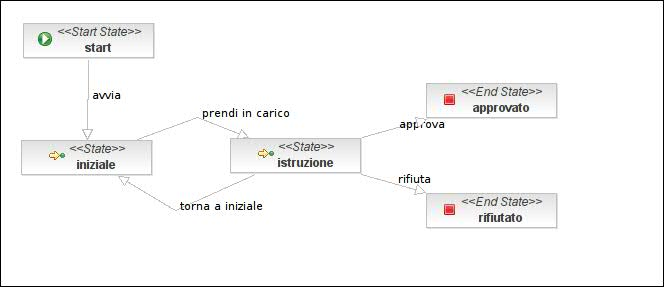
\includegraphics[scale=0.5]{workflow} 
  \caption[workflow]{Grafico di un workflow \label{fig:workflow}}
\end{figure}

Nel flusso di esempio sono presenti cinque stati: \textit{start}, \textit{iniziale}, \textit{istruzione}, \textit{approvato} e \textit{rifiutato}.  Nella definizione di un nuovo flusso conviene rammentarsi di aderire ad alcune convenizioni stabilite da Plitvice kit: ad esempio conviene utilizzare come nomi degli stati  
\begin{inparaenum}[\itshape a\upshape)]
\item  solo caratteri minuscoli e possibilemente \item preferire gli aggettivi ai sostantivi. 
Ogni workflow deve necessariamente \item iniziare  con lo stato \textit{start} che deve prevedere  \item un'unica transizione denominata \textit{avvia}.
Tornando all'esempio le altre transizioni sono \textit{prendi in carico}, \textit{torna a iniziale}, \textit{approva} e \textit{rifiuta}; da notare la convenzione di utilizzare \item dei verbi in modo imperativo per definire le transizioni. 
Infine alcuni stati sono detti terminali perché una volta raggiunti non è più possibile lasciarli (nell'esempio \textit{approvato} e \textit{rifiutato}).
\end{inparaenum}


\section{Tabella di marcia}
Le applicazioni Regola kit possono essere configurate per la gestione di workflow semplicemente aggiungendo una dipendenza al modulo \textit{plitvice-workflow}. Predisporre invece un proprio gestore di flussi richiede diverse operazioni:

\begin{itemize*}
\item definire un Workflow
\item creare un WorkflowRepository
\item definire un Ruolo con i relativi Diritti
\item progettare una classe di Visibilità
\item creare un AuthenticationManager
\item progettare il documento
\item progettare la classe WorkflowManager
\item progettate la classe WorkflowActions
\end{itemize*}

In effetti sembrano parecchie ma in realtà sono piuttosto veloci da approntare perché Plitvice kit fornisce tutte le classi di basi necessarie ad un'applicazione reale: ad esempio sono già previsti i supporti per i WorkflowRepository su database o in memoria tramite mock.
Nel corso della presentazione verranno toccati tutti i punti dell'elenco e si provvederà a realizzare un esempio concreto per la gestione di un Workflow denominato \textit{accordo} in grado di gestire un documento di tipo Accordo.

\section{Workflow}
Plitvice kit utilizza JBoos jBPM internamente per la gestione dei Workflow. La definizione di un Workflow avviene quindi mediante un file XML che raccoglie gli stati e le transizioni. Per chi utilizza Eclipse è disponibile un comodo plug in visuale che può essere di un qualche aiuto nella progettazione del workflow. Affinché la definizione sia fruibile da Plitvice kit è necessario che si attenga alle seguenti convenzioni:

\begin{itemize*}
\item il file xml contenente la definizione deve essere salvato nella posizione  src/main/resources/workflows/nomeflusso/processdefinition.xml

\item il nodo iniziale di ogni flusso deve chiamarsi \textit{start} 

\item dal nodo iniziale deve uscire solo una transizione denominata \textit{avvia}

\item ogni transizione che prevede una modifica di database deve essere associata ad un'azione gestita dalla classe PersistenceAction come nel frammento di definizione seguente:
\begin{xml}
<state name="iniziale">
    <transition to="istruzione" name="prendi in carico">
      <action class="it.kion.plitvice.workflow.service.impl.PersistenceAction"></action>
    </transition>
  </state>
\end{xml}

\item i nomi degli stati devono contenere solo caratteri minuscoli e possibilmente essere espressi mediante aggettivi (tipo iniziale, approvato, ecc.)

\item i nomi delle transizioni devono contenere solo caratteri minuscoli e possibilmente essere espressi mediante verbi nel modo imperativo (tipo accetta, rifiuta, ecc.)

\end{itemize*}


\section{WorkflowRepository}
Un WorkflowRepository è un'entità di modello che consente di accedere a tutti i Workflow disponibili per l'applicazione in modo che i WorkflowManager possano, conoscendone solo il nome, accedere a tutte le proprietà di un flusso, compresa la definizione. 
Generalmente il repository si concretizza semplicemente in una tabella di database che elenchi i diversi workflow e ne raccolga gli attributi. Plitvice kit prevede una classe per gestire questa tabella,  WorkflowRepositoryHibernate.
Alternativamente, spesso impiegati per la fase di test, si può creare un repository in memoria popolato mediante configurazione di Spring (si veda ad esempio WorkflowRepositoryMock).

\section{Autorizzazioni}

L'autorizzazione su un workflow consiste nello stabilire se l'identità correntemente assunta dell'utente autenticato possa o meno segnalare una certa transizione oppure abbia i permessi per elencare i documenti in un certo stato. Lo schema delle autorizzazioni è quello definito nel modulo plitvice security che prevede il concetto di Ruolo a cui fa capo una collezione di diritti (Diritto); questi ultimi possono essere di natura applicativa oppure relativi ai workflow. Infine questi ultimi si distinguono per occuparsi degli stati oppure delle transizioni.

Gli elementi comuni ad ogni diritto sono un identificativo unico (un intero) ed un Ambito che rappresenta un partizionamento su base applicativa; ad esempio esiste l'ambito dei tirocini che raccoglie tutti i diritti relativi alla grande area della gestione dei tirocini. Inoltre tutti i diritti fanno riferimento ad un'Entità, ovvero un elemento del modello con un ciclo di vita ampio secondo i dettami del Domain Driven Development. L'elenco delle Entità è persistito su database e a ciascuna è assegnato un identificativo univoco. I diritti relativi a workflow contengono invece sempre l'indicazione del flusso.\footnote{Attualmente dato un workflow discende una ed una sola entità per cui basterebbe l'indicazione del flusso per risalire inequivocabilmente all'entità; comunque al momento in cui questo manuale è redatto, sia l'id dell'entità che il nome del flusso devono essere specificate in modo congruente.}

I diritti di workflow di tipo transazione prevedono la possibilità di segnalare una specifica transazione. Il default, ovvero in caso di assenza di uno specifico diritto, la transazione non può essere segnalata da nessuno.
I diritti di workflow di tipo stato consentono di elencare tutti i documenti che si trovino in quello stato. In assenza di un particolare diritto chiunque può richiedere l'elenco completo dei documenti per quel certo stato. Comunque anche le identità sprovviste di diritti di elencazione possono riuscire ad ottenere gli elenchi dei documenti utilizzando un meccanismo apposito; si rimanda alla proprietà vincoloLettura di AutorizzazioneUtente e l'interfaccia Visibilità per dettagli in merito.

Le autorizzazioni sono abilitate o disabilitate tramite un aspetto di Spring; per attivarle  basta aggiungere le seguenti righe in un file di configurazione di bean:
\begin{xml}
<!-- Enable @AspectJ support -->
<aop:aspectj-autoproxy proxy-target-class="false" />
  
<bean class="it.kion.plitvice.autorizzazioni.WorkflowManagerAuthentication" >
   <property name="authentication" ref="authenticationManager" />
</bean>
\end{xml}

\section{Il documento}
Un workflow documentale è destinato alla gestione di un documento, ad esempio potrebbe rappresentare i passi necessari e le persone (o gli uffici) coinvolti nel processo ufficiale di produzione di una pratica. 
In questo contesto il termine documento si riferisce ad  una classe Java, in particolare  un'entità di modello applicativo per la quale è eventualmente stato definito un  Model Pattern di Regola kit. Nel corso di questo capitolo, come si è detto, presenteremo un esempio concreto il cui documento è  l'entità Accordo:

\begin{java}
package it.kion.plitvice.workflow.model;

import it.kion.plitvice.workflow.service.impl.AccordoWorkflowActions;
import it.kion.plitvice.workflow.service.impl.AccordoWorkflowActions.Stati;

import java.io.Serializable;

public class Accordo implements Serializable {

  private Stati stato = Stati.start;
  private Long id = null;
  
  public void setStato(Stati stato) {
    this.stato = stato;
  }

  public Stati getStato() {
    return stato;
  }

  public void setId(Long id) {
    this.id = id;
  }

  public Long getId() {
    return id;
  }
  
}
\end{java}

Durante la fase di progettazione del documento deve essere tenuta in considerazione la relazione forte che lega  il documento al workflow che lo gestisce; in qualsiasi momento del ciclo di vita del documento deve esistere un modo (un algoritmo)  che partendo da un'istanza del documento sappia determinare il workflow di riferimento unitamente allo stato in cui il workflow si trova.  In altri termini lo stato del workflow deve essere desumibile attraverso il documento stesso, o perché lo contiene direttamente  o perché contiene gli elementi per recuperare da un database lo stato del flusso. 
Nel nostro semplice esempio lo stato del flusso è semplicemente una proprietà del documento.

Il WorkflowManager consentirà di effettuare delle selezioni dalla popolazione di tutti i documenti gestiti tramite flussi: sarà in particolare possibile ottenere l'elenco di tutti i documenti che si trovino in un certo stato oppure gestiti da un certo workflow. Per effettuare questo genere d'interrogazioni è stato esteso il meccanismo di ModelPattern con due annotazioni, @Stati e @Workflow.

\begin{java}

package it.kion.plitvice.workflow.dao;

import it.kion.plitvice.workflow.model.Workflow;
import it.kion.plitvice.workflow.pattern.Stati;

import org.regola.model.ModelPattern;

public class AccordoPattern extends ModelPattern {

  String[] inStati = new String[] {};
  private Workflow flusso;

  @Stati()
  public String[] getInStati() {
    return inStati;
  }

  public void setInStati(String[] inStati) {
    this.inStati = inStati;
  }
  
  @it.kion.plitvice.workflow.pattern.Workflow
  public Workflow getFlusso() {
    return flusso;
  }

  public void setFlusso(Workflow flusso) {
    this.flusso = flusso;
  }
  
}
\end{java}

Tanto per avere un'idea fin da subito del funzionamento del ModelPattern nel contesto dei workflow può risultare utile l'esempio seguente che richiede al gestore del flusso tutti i documenti che si trovino nello stato \textit{iniziale} mediante una chiamata al metodo elencoProcessiInStati. 

\begin{java}
AccordoPattern pattern = new AccordoPattern();
pattern.setInStati(new String[] { "iniziale" });
    
// recupero il documento gestito dal flusso
List<Accordo> accordi = 
 accordoManager.elencoProcessiInStati(pattern, autNicola);
\end{java}


Come si vede prima si imposta AccordoPattern con lo stato d'interesse (iniziale) e poi lo si passa al metodo elencoProcessiInStati


\section{WorkflowManager: funzionamento}
Nel livello di servizio, assieme agli altri Business Delegate, i Service Facade ed in generale tutte le classi che consentono di fruire del modello, trovano collocazione i WorkflowManager; si tratta di Manager nel senso indicato da Regola kit che offrono un'interfaccia comune per la gestione dei flussi di lavoro. 

\begin{java}
public interface WorkflowManager
<D extends Serializable, ID extends Serializable> 
extends GenericManager<D,ID> {

  List<D> elencoProcessiInStati(ModelPattern pattern, AutorizzazioniUtente utente);
  int countProcessiInStati(ModelPattern pattern, AutorizzazioniUtente utente);
  
  String segnala(D processo, String transizione,AutorizzazioniUtente utenti) throws ProcessoNonValidoException, TransizioneNonValidaException;
  
  String avviaFlusso(Workflow flusso,Object documentoIniziale,AutorizzazioniUtente utenti);
  String avviaFlusso(Object documentoIniziale,AutorizzazioniUtente utenti);

  List<String> transizioniDisponibili (D processo, AutorizzazioniUtente utente);

  public List<String> elencoStati(D processo);


  Workflow[] elencoFlussiGestiti();

}
\end{java}


Ogni WorkflowManager si occupa di un solo tipo di documento D (un entità serializzabile e persistibile su database) la cui chiave d'identificazione è del tipo ID. Ricordo che il tipo D (il documento) può essere associato ad uno o più workflow tutti gestiti dallo stesso WorkflowManager; per sapere quali sono i flussi di lavoro gestiti da un WorkflowManager bisogna invocare il metodo   elencoFlussiGestiti(). Non bisogna dimenticare che se la classe D del documento può essere gestita da diversi flussi la singola istanza è gestita solo da uno ed un solo flusso; ovvero se un'istanza inizia il suo percorso all'interno di un workflow non può abbandonarlo più. Da questo deriva che data istanza di D è possibile determinare in modo univoco il flusso che la gestisce ed in questo modo è utilizzata all'interno degli altri metodi di WorkflowManager. 
Un'altra considerazione generale riguarda il sistema di autorizzazione che verifica le credenziali dell'utente collegato prima di consentire l'elencazione di documenti in un certo stato oppure la segnalazione di una transizione; molti metodi di WorkflowManager richiedono il passaggio di un DTO chiamato AutorizzazioniUtente che consente di individuare con esattezza l'identità selezionata dall'utente corrente ed applicare i criteri di autorizzazione. Per maggiori dettagli si rimanda al modulo plitvice security.

Il primo metodo da invocare per avviare un nuovo servizio è avviaFlusso() al quale si può eventualmente passare un oggetto preliminare che contenga le informazioni necessarie per creare il documento da inserire nel flusso. Naturalmente documento e oggetto preliminare possono coincidere se lo si ritiene conveniente. Come si è visto data un'istanza di documento  è possibile risalire al flusso; nel momento che precede la creazione di un nuovo flusso però quell'istanza non esiste per cui è necessario specificare al  metodo avviaFlusso() quale workflow utilizzare tra quelli gestiti da uno specifico WorkflowManager. Se si omette questa indicazione sarà utilizzato il primo workflow tra quelli gestiti.

Una volta avviato un flusso è possibile elencare tutti i documenti che si trovino in un certo stato tramite il metodo  elencoProcessiInStati() passandogli come parametro un ModelPattern come indicato nel paragrafo precedente.

Avuto un documento in un certo stato è possibile sapere quali siano le transizioni che gli sono consentite dall'identità correntemente assunta tramite il metodo  transizioniDisponibili().

Infine per segnalare una transizione (cioè cambiare stato) si richiami il metodo  segnala().


\section{WorkflowManager: progettazione}

La creazione di un servizio di workflow si limita alla creazione di un'interfaccia che estenda WorkflowManager e nel darne un'implementazione di massima.

\begin{java}

public interface AccordoWorkflowManager 
 extends WorkflowManager<Accordo, Long> {
}

public class AccordoWorkflowManagerImpl 
extends WorkflowManagerImpl<Accordo, Long> 
implements AccordoWorkflowManager 
{

  public AccordoWorkflowManagerImpl(GenericDao<Accordo, Long> dao) {
    super(dao);
    setFlussiGestiti(new String[] { "accordo" });
  }

  @Override
  protected void addProcessVariable(ProcessInstance instance) {
    // TODO Auto-generated method stub
  }

  @Override
  public Workflow flowForDocument(Accordo documento) {
    return repository.findByName(flussiGestiti[0]);
  }
  
}

\end{java}


I metodi di cui occuparsi nell'implementazione sono il costruttore in cui specificare i workflow gestiti da questo WorkflowManager, nell'esempio solo uno di nome \textit{accordo} che per quando indicato nelle convenzioni relative alle definizioni dei workflow deve trovarsi nella posizione src/main/resources/workflows/accordo/processdefinition.xml.
Il metodo flowForDocument() consente di individuare a quale flusso sia associata l'istanza del documento; nel nostro esempio ogni istanza è gestita da un solo workflow.
Infine addProcessVariable() consente di inserire delle variabili da utilizzare all'interno delle action durante le segnalazioni. Nell'esempio non è impiegato questo metodo.
Il file di definizione di Spring per le classi appena create deve assomigliare al seguente frammento:

\begin{xml}
<bean id="accordoActions" class="it.kion.plitvice.workflow.service.impl.AccordoWorkflowActions" >
  <property name="dao" ref="accordoDao" />
</bean>
  
<bean id="accordoManager" class="it.kion.plitvice.workflow.service.impl.AccordoWorkflowManagerImpl" >
   <constructor-arg>
      <ref bean="accordoDao"/>
    </constructor-arg>
        <property name="actions" ref="accordoActions" />
    <property name="repository" ref="workflowRepositoryMock" />
    <property name="visibilitaFactoryChain" ref="visibilitaFactoryChain" />
</bean>
\end{xml}

Come si può osservare le dipendenze di ogni WorkflowManager sono la classe di actions che si occupa come si vedrà di definire le logiche di persistenza, un elemento di modello chiamato repository che si occupa di fornire l'accesso a tutte le difinizioni dei workflow disponibili per l'applicazione ed infine una  visibilitaFactoryChain che è intimamente legata con i criteri di applicazione delle autorizzazioni per cui si rimanda alla documentazione del modulo plitvice security per i dettagli.

\section{WorkflowActions}

La persistenza del workflow (e del documento a cui si riferisce) può essere completamente personalizzata tramite la progettazione di una classe che estenda WorkflowActions; i metodi di questa classe saranno richiamati (internamente da WorkflowManager )  al momento di attraversare una transizione o quando è richiesto un elenco di documenti. 
Molto probabilmente la vostra classe di action avrà un dao di Regola kit tra le dipendenze e lo userà nei modi consueti finendo per assomigliare ad una versione complessa di quella presentata qui di seguito:

\begin{java}
public class AccordoWorkflowActions 
   extends WorkflowActions<Accordo> {
  
  public enum Stati {
    start, iniziale, istruzione, approvato, rifiutato
  };
  
  private AccordoDao dao;
  
  public List<Accordo> elencoProcessiInStati(Workflow flusso, String [] stati, ModelPattern p, AutorizzazioniUtente utente)
  {
    log.info("elencoProcessiInStati=");
    return getDao().find(p); 
  }
  
  public int countProcessiInStati(Workflow flusso, String [] stati, ModelPattern p, AutorizzazioniUtente utente) 
  {
    log.info("countProcessiInStati=");
    return getDao().count(p);
  }
  
    @Override
  @StatoCorrente()
  public String getStatoCorrente(Accordo documento)
  {
    return documento.getStato().toString();
  }
  
  @Override
  public String avviaFlusso(Object documentoIniziale, AutorizzazioniUtente utente) {
    log.info("avviaFlusso");
    
    Accordo accordo = new Accordo();
    
    accordo.setId(1l);
    accordo.setStato(Stati.iniziale);
    
    dao.save(accordo);
    
    return Stati.iniziale.toString();
  }
  
  @Transizione("prendi in carico")
  public void segnalaPrendiInCarico(Accordo documento, String transizione, AutorizzazioniUtente utente) {
    documento.setStato(Stati.istruzione);
    dao.save(documento);
  }

  @Transizione("torna a iniziale")
  public void segnalaTornaAIniziale(Accordo documento, String transizione, AutorizzazioniUtente utente) {
    documento.setStato(Stati.iniziale);
    dao.save(documento);
  }

  @Transizione("approva")
  public void segnalaApprova(Accordo documento, String transizione, AutorizzazioniUtente utente) {
    documento.setStato(Stati.approvato);
    dao.save(documento);
  }

  @Transizione("rifiuta")
  public void segnalaRifiuta(Accordo documento, String transizione, AutorizzazioniUtente utente) {
    documento.setStato(Stati.rifiutato);
    dao.save(documento);
  }

  public void setDao(AccordoDao dao) {
    this.dao = dao;
  }

  public AccordoDao getDao() {
    return dao;
  }

}

\end{java}


Nel progettare la classe action bisogna implementare dei metodi la cui firma è nota ( ProcessiInStati,  countProcessiInStati, getStatoCorrente() e avviaFlusso()) ed aggiungere anche dei metodi (dal nome libero e la firma predeterminata)  da associare ad ogni transizione gestita.
ElencoProcessiInStati e  countProcessiInStati forniscono la base materiale per l'estrazione dal database dei documenti nello stato richiesto. 
Il metodo  getStatoCorrente() che consente di determinare, dato un documento, il suo stato attuale.
Infine avviaFlusso() provvede a creare un flusso nuovo dato un oggetto preliminare.
Inoltre devono essere creati tanti metodi quante sono le transizioni che abbisognano di persistenza da marcare con l'annotazione @Transizione ed il nome della transazione. Il sistema provvederà a chiamare automaticamente questi metodi al momento della segnalazione, subito dopo che lo stato logico del flusso è stato aggiornato.



% -----------BIBLIOGRAFIA

%\begin{thebibliography}{9}
%\bibitem{lamport94}
%  Leslie Lamport,
%  \emph{\LaTeX: A Document Preparation System}.
%  Addison Wesley, Massachusetts,
%  2nd Edition,
%  1994.
%\end{thebibliography}

\bibliographystyle{alpha}
\bibliography{main}



% -----------INDICE
\printindex

\end{document}
